\documentclass[final]{beamer} % beamer 3.10: do NOT use option 
\mode<presentation> {
	\usetheme{prometheus}
}
\setbeamertemplate{caption}[numbered]

\usepackage[english]{babel}
\usepackage[latin1]{inputenc}
\usepackage{amsmath,amsthm, amssymb, latexsym}
\usefonttheme[onlymath]{serif}
\boldmath
\usepackage[orientation=landscape,size=a1,debug]{beamerposter}
\usepackage{float}    
\usepackage{subcaption}              % e.g. for DIN-A0 poster
\usepackage{siunitx}
\usepackage[noabbrev,capitalize,nameinlink]{cleveref}
\title[Fancy Posters]{Prometheus AI}
\author{Sean Stappas --- Supervised by Prof. Vybihal}
\institute[RWTH Aachen University]{}
\date{Jul. 31th, 2007}

\newlength{\columnheight}
\setlength{\columnheight}{100cm}
\newcommand{\code}[1]{\texttt{#1}}

\begin{document}
	\begin{frame}
		\begin{columns}
			\begin{column}{.33\textwidth}
				\parbox[t][\columnheight]{\textwidth}{
				\begin{block}{Introduction \& Background}
					\parbox{0.99\textwidth}{
						\textbf{Prometheus} is an AI system designed to control and coordinate multiple \textbf{robots} based on their sensor data. Its architecture is loosely inspired from the structure of the human brain, and is composed of the following four layers: the \textbf{Neural Network (NN)}, the \textbf{Knowledge Node Network (KNN)}, the \textbf{Expert System (ES)}, and the \textbf{Meta Reasoner (META)}. The \textbf{Neural Network} layer is the interface to the robots' sensors and provides informational tags to the KNN.}
				
					\begin{figure}[!htb]
						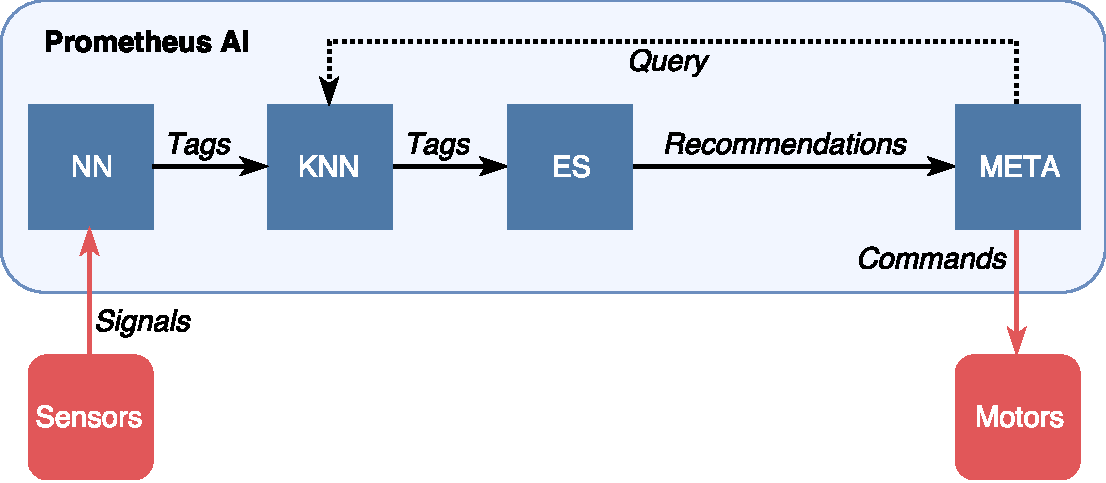
\includegraphics[width=0.99\textwidth]{figures/ai_model_labeled.pdf}
						\caption{Prometheus AI model with labeled input and output.}
						\label{model_labeled}
					\end{figure}
				
					\parbox{0.99\textwidth}{The \textbf{Knowledge Node Network} layer is the analog to \textbf{memory} in the human brain. It takes in the tags provided by the NN and outputs tags based on its knowledge. It consists of interconnected \textbf{Knowledge Nodes} (KNs), which are abstract structures representing \textbf{memories} and their connections to other memories. There are many concepts associated with KNs, such as \textbf{activation}, \textbf{firing}, \textbf{strength}, \textbf{aging} and \textbf{belief}. The KNN has 4 ways of searching to fire KNs and activate tags: \textbf{direct}, \textbf{forward}, \textbf{backward} and \textbf{lambda}.}
					
					\begin{figure}[!htb]
						\centering
						\begin{subfigure}[!htb]{0.49\columnwidth}
							\centering
							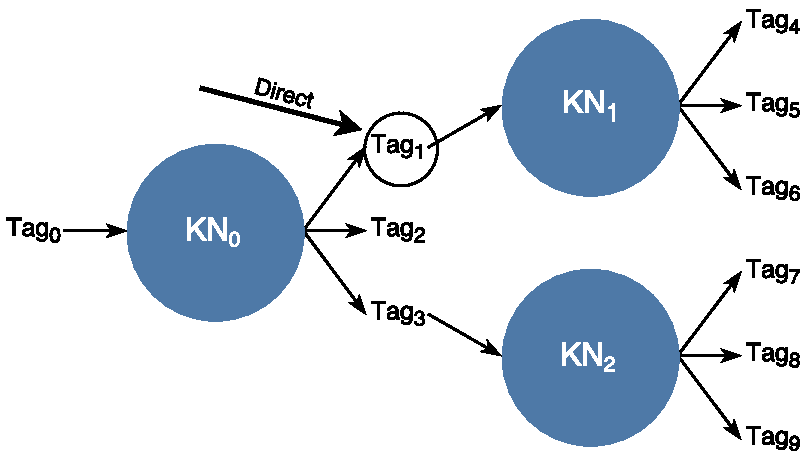
\includegraphics[height=2.8in]{figures/direct_search.pdf}
							\caption{Direct searching.}
						\end{subfigure}
						\begin{subfigure}[!htb]{0.49\columnwidth}
							\centering
							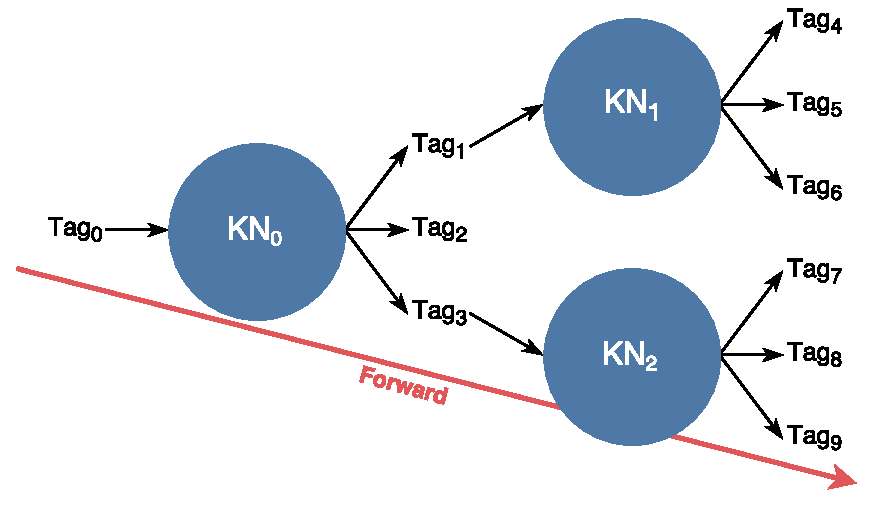
\includegraphics[height=2.8in]{figures/forward_search.pdf}
							\caption{Forward searching/thinking.}
							\label{think_forwards}
						\end{subfigure}
						\bigskip
						\begin{subfigure}[!htb]{0.49\columnwidth}
							\centering
							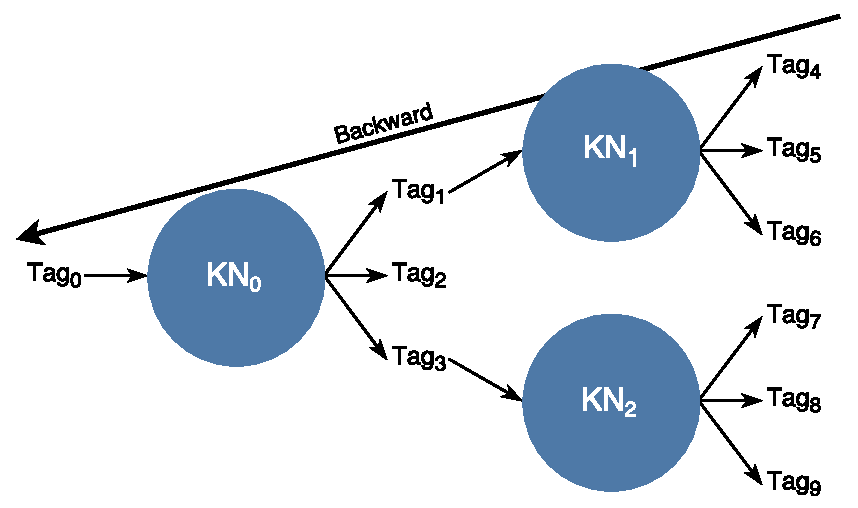
\includegraphics[height=2.8in]{figures/backward_search.pdf}
							\caption{Backward searching/thinking.}
							\label{think_backwards}
						\end{subfigure}
						\begin{subfigure}[!htb]{0.49\columnwidth}
							\centering
							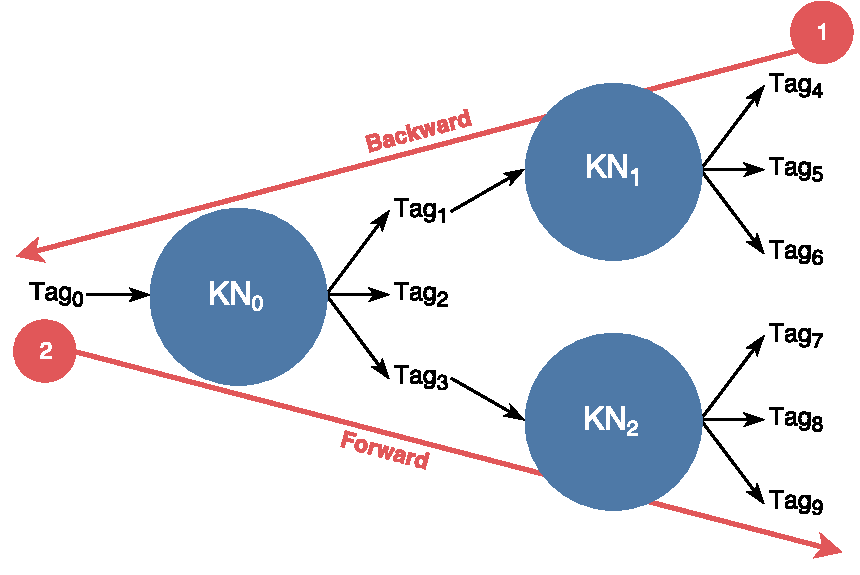
\includegraphics[height=2.8in]{figures/lambda_search.pdf}
							\caption{Lambda searching/thinking.}
							\label{think_lambda}
						\end{subfigure}
						\caption{Methods of searching and thinking in the KNN.}
					\end{figure}
					
					\parbox{0.99\textwidth}{The \textbf{Expert System} layer is a basic logic reasoner. It is not aware of its current reality or any context. It takes in the tags provided by the KNN and interprets them as either \textbf{facts}, \textbf{recommendations} or \textbf{rules}. Based on these rules, it performs a thinking routine to activate recommendations and provide them to the Meta Reasoner.
						
					\begin{figure}[!htb]
						\centering
						\begin{subfigure}[!htb]{0.4\columnwidth}
							\centering
							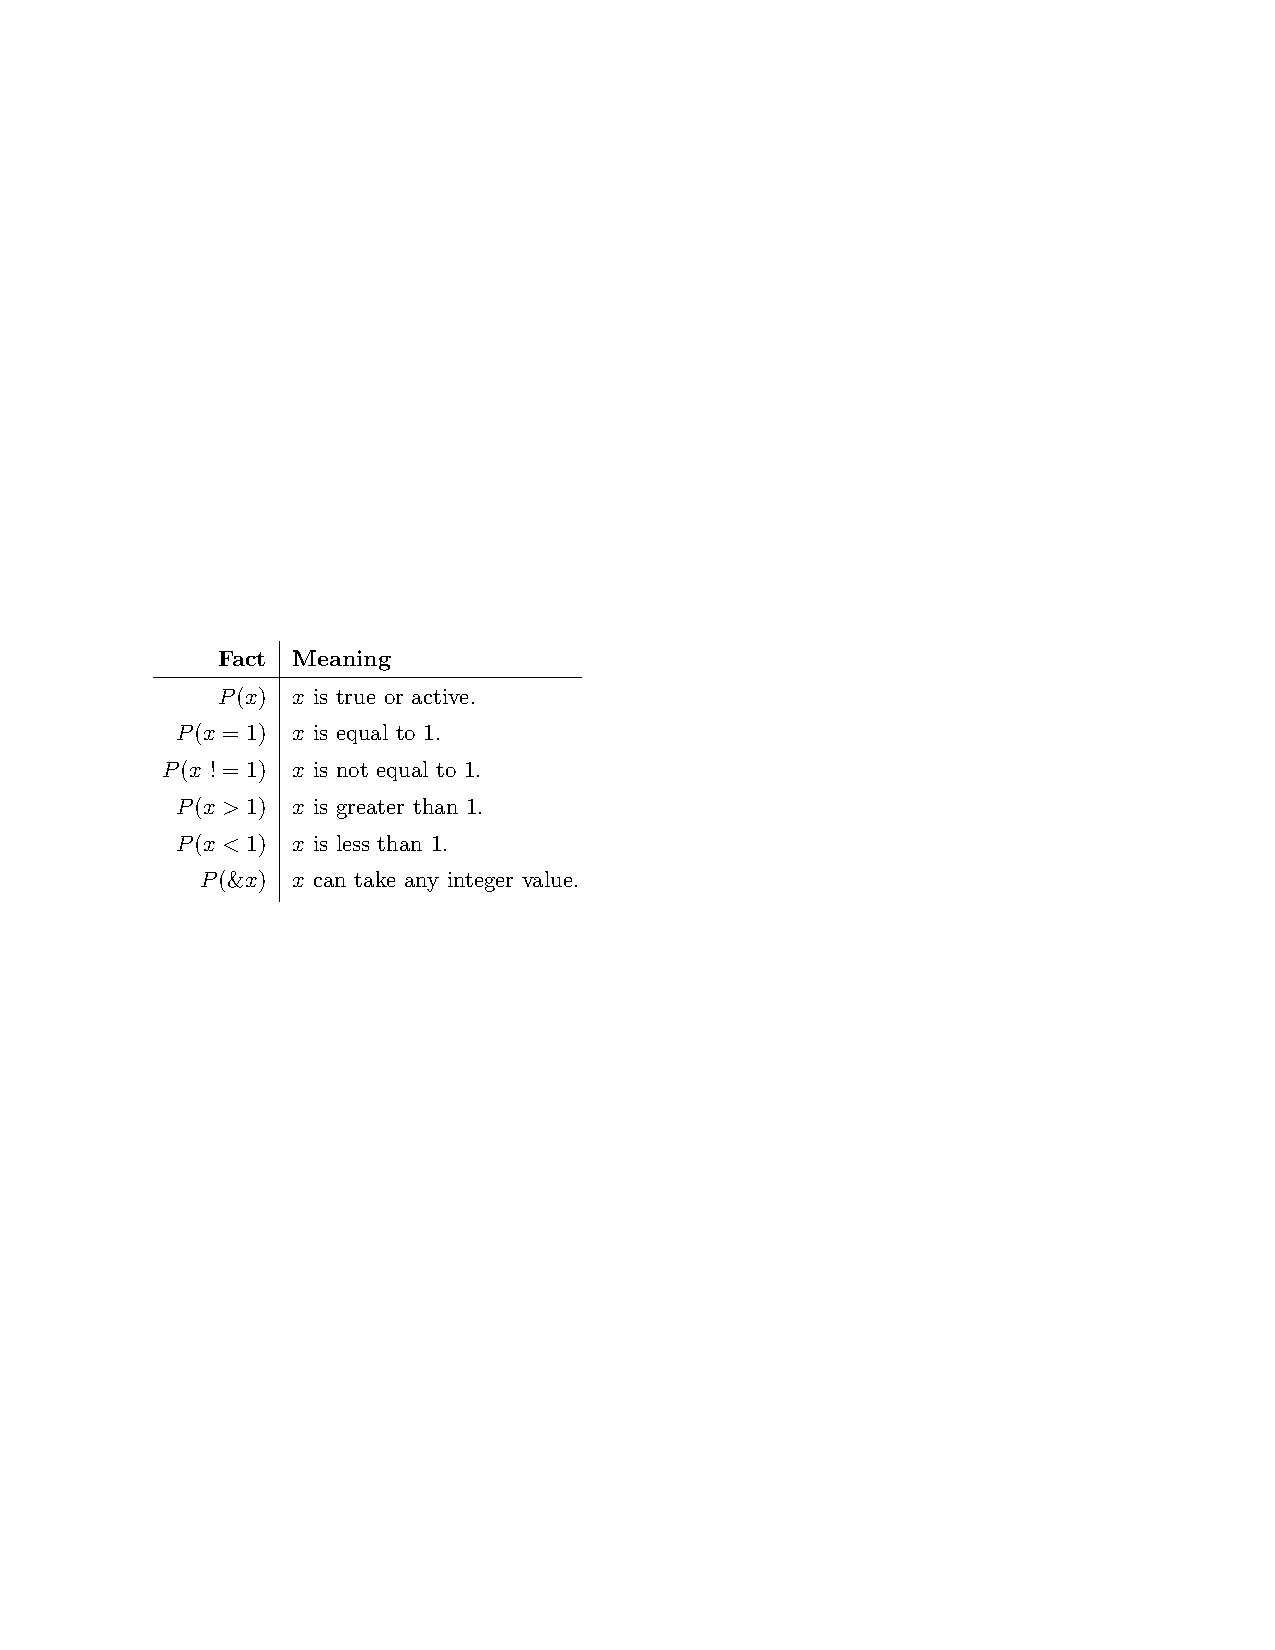
\includegraphics[height=2.5in]{figures/fact_examples.pdf}
							\caption{Examples of simple facts in the ES.}
						\end{subfigure}
						\begin{subfigure}[!htb]{0.58\columnwidth}
							\centering
							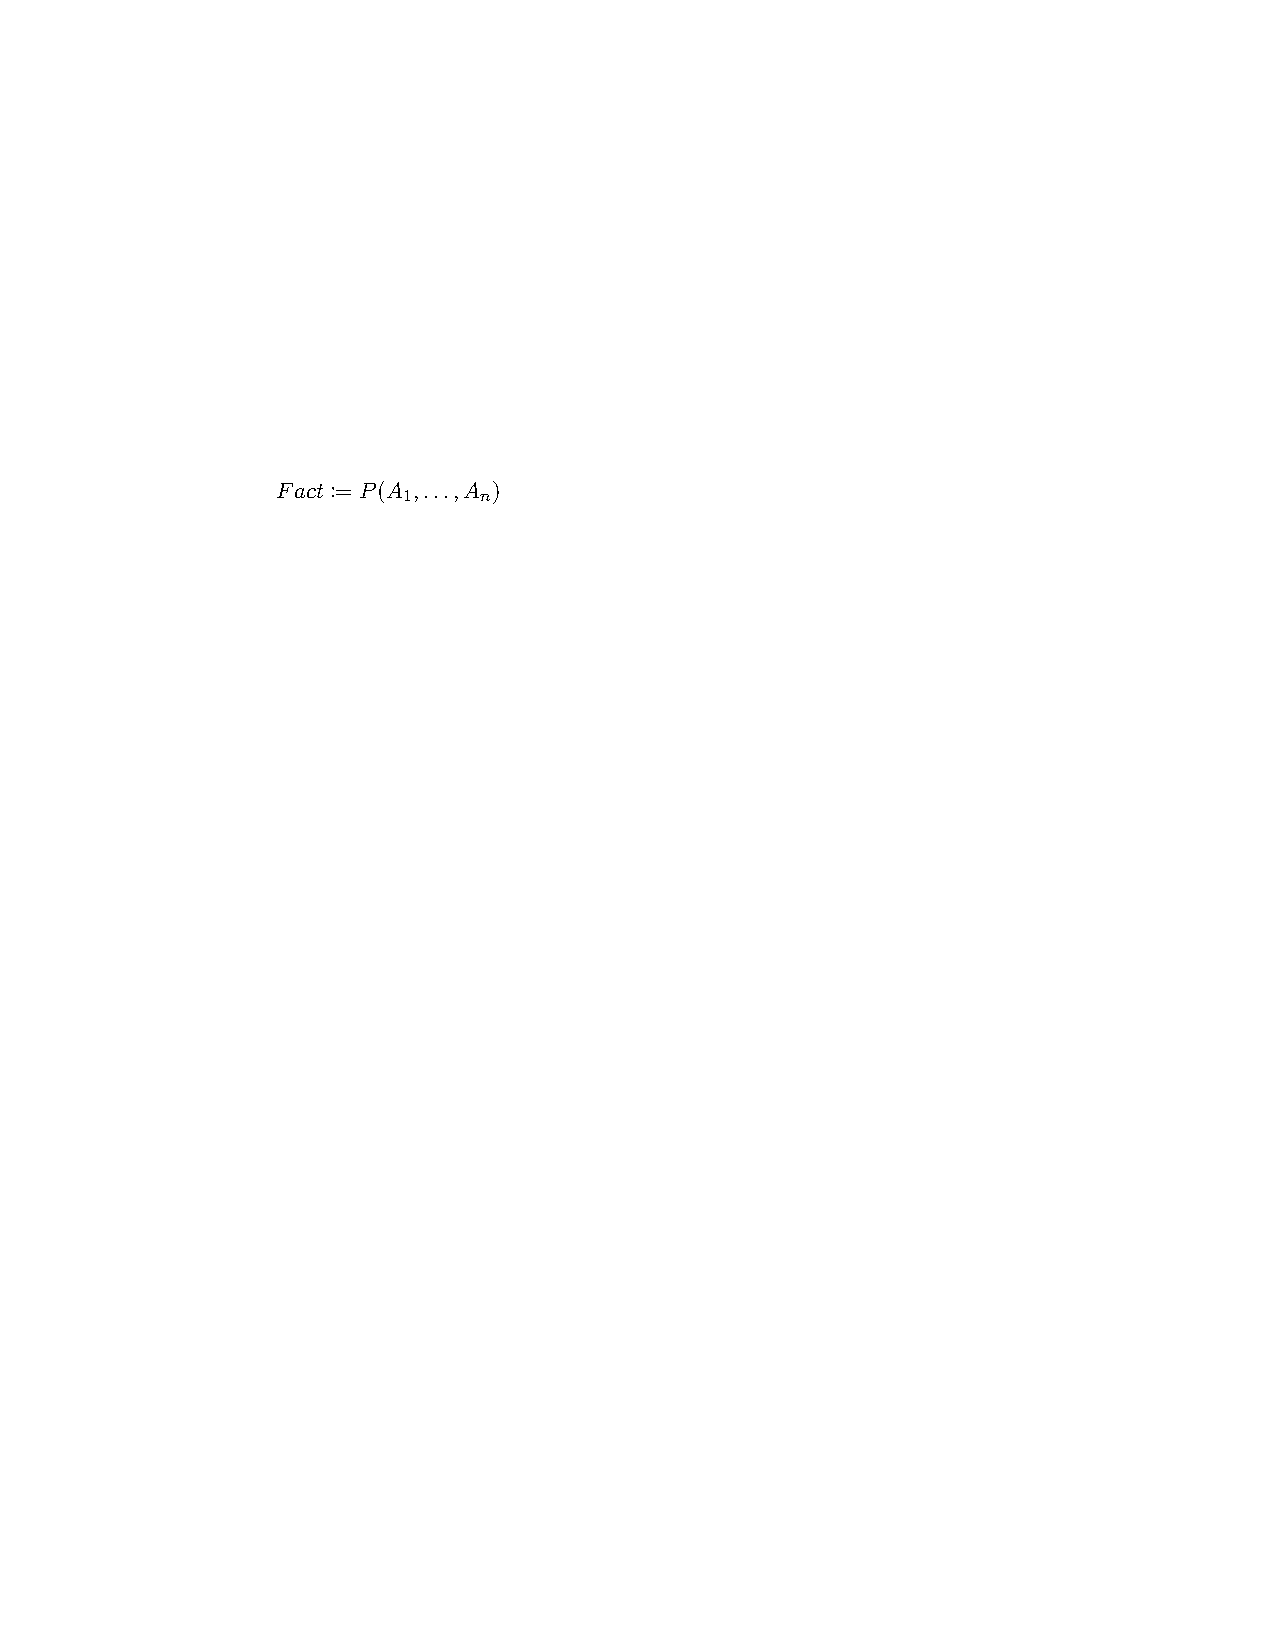
\includegraphics[width=0.5\columnwidth]{figures/fact.pdf}
							\caption{The form of a fact in the ES. $P$ is a predicate, and $A_i$ is an argument.}
							
							\vspace{1ex}
							
							
\includegraphics[width=0.7\columnwidth]{figures/recommendation.pdf}
							\caption{The form of a recommendation in the ES. $P$ is a predicate, and $A_i$ is an argument..}
							
							\vspace{1ex}
							
							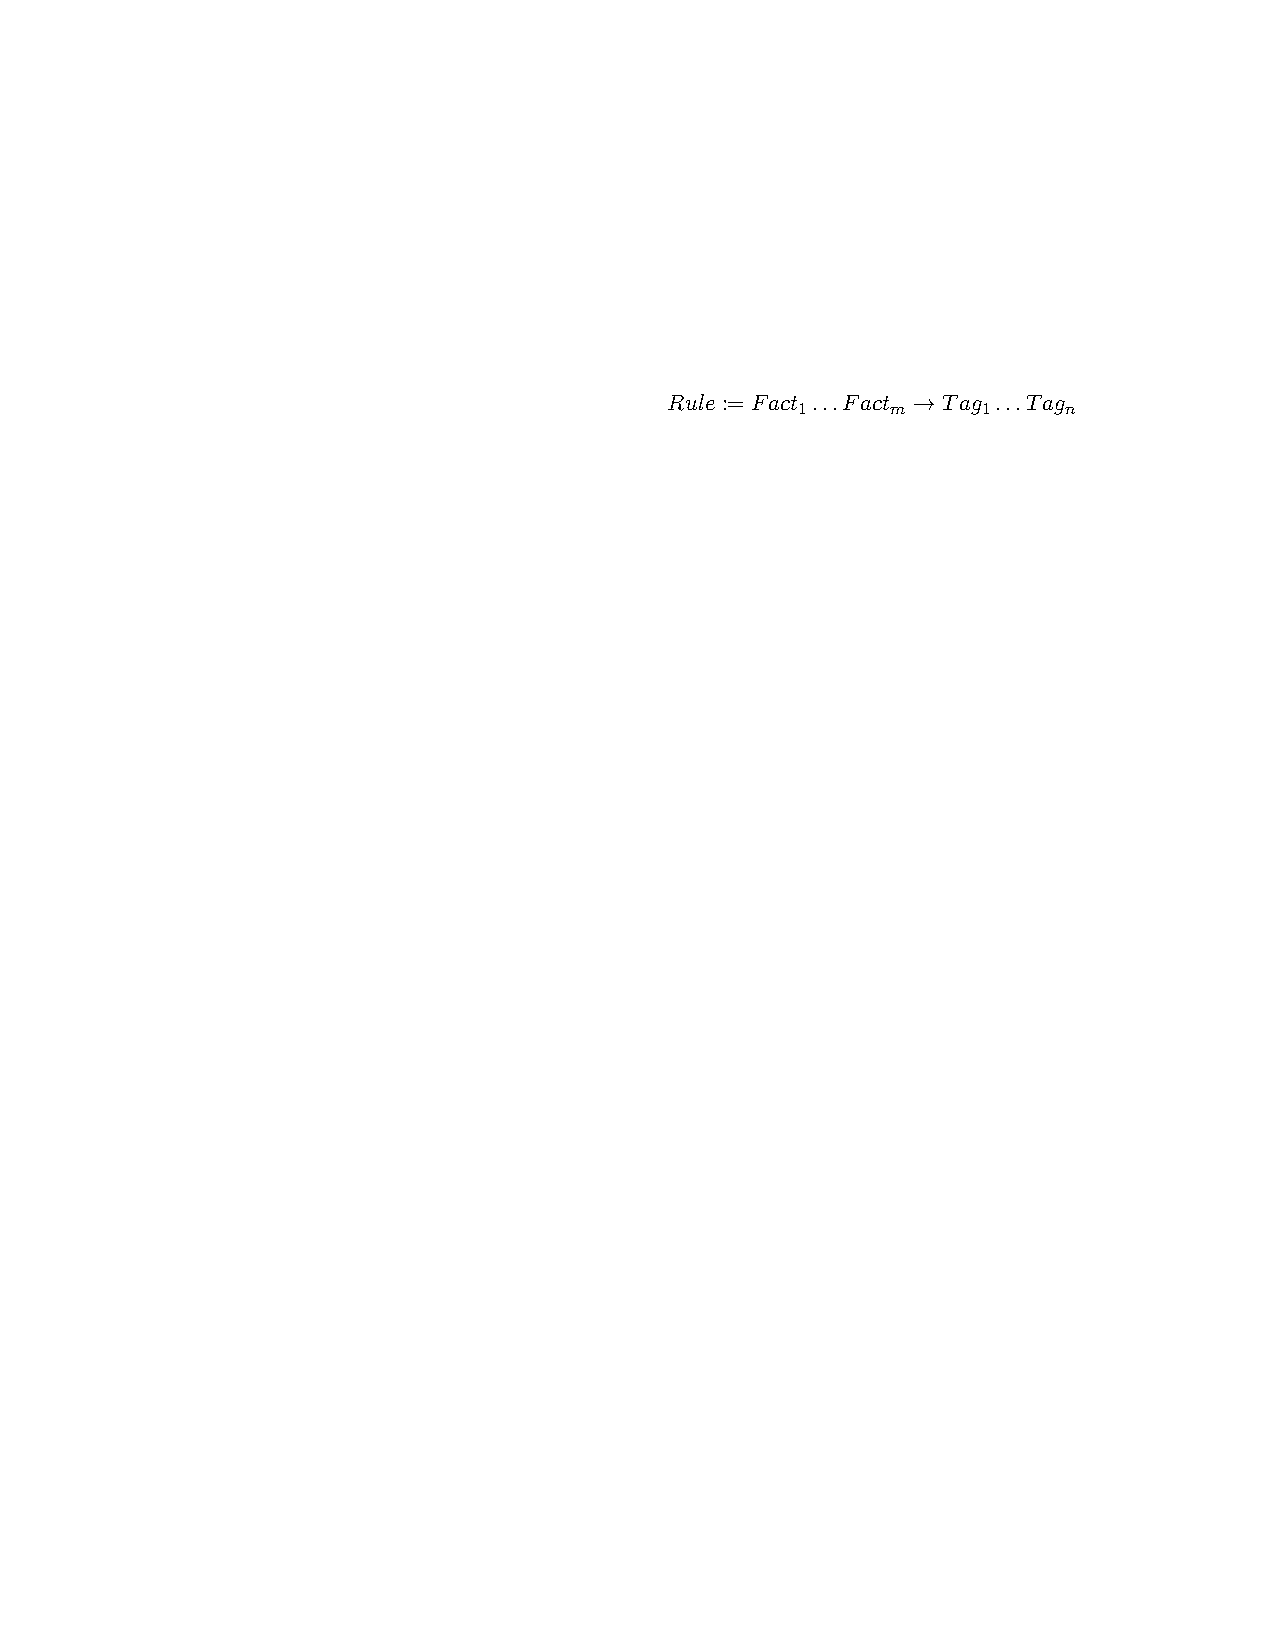
\includegraphics[width=\columnwidth]{figures/rule.pdf}
							\caption{The form of a rule in the ES, with $m$ input facts and $n$ output tags. The output tags must either be facts or recommendations.}
						\end{subfigure}
						\caption{Facts, recommendations and rules in the ES.}
					\end{figure}
					
					
					The \textbf{Meta Reasoner} represents high-level reasoning in the human brain. It is aware of its environment and context, and makes informed decisions to send actuator commands to the robots.}
				\end{block}
			}
			\end{column}
			\begin{column}{.33\textwidth}
				\parbox[t][\columnheight]{\textwidth}{
				
				\begin{block}{Problem}
					\parbox{0.99\textwidth}{
					There are two main assigned tasks over the past two semesters:
					\begin{enumerate}
						\item Design and implement the \textbf{Expert System} and \textbf{Knowledge Node Network} in Java.
						\item Supervise undergraduate students working on Prometheus.
				\end{enumerate}}
				\end{block}
					
				\begin{block}{Design \& Implementation}
					\parbox{0.99\textwidth}{
					The high-level \textbf{Prometheus} interface has dependencies on the \code{NeuralNetwork}, \code{KnowledgeNodeNetwork}, \code{ExpertSystem} and \code{MetaReasoner} interfaces. The \code{KnowledgeNodeNetwork} and \code{ExpertSystem} layers are the ones that are currently implemented. The code base was designed to be \textbf{efficient}, \textbf{modular} and easily \textbf{testable}. The \textbf{tags} used throughout the system are implemented using a \code{Tag} Java class, with \code{Predicate} and \code{Rule} subclasses. The \code{Predicate} class is a superclass of the \code{Fact} and \code{Recommendation} and represents the possible output tags of a rule.}
				
					\begin{figure}
						\centering
						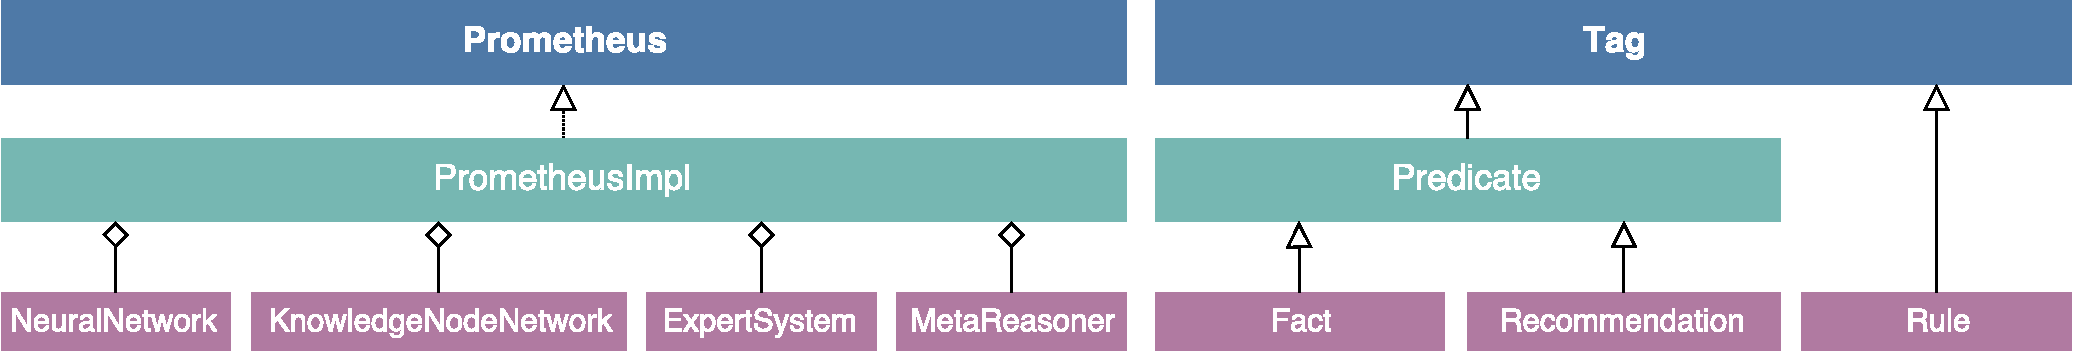
\includegraphics[width=0.99\textwidth]{figures/uml_combined_1.pdf}
						\caption{UML diagrams of the Prometheus and Tag packages.}
					\end{figure}			
				
					\parbox{0.99\textwidth}{
					The most important method in the \textbf{Expert System} is \code{think()}, which executes \textbf{thinking cycles} and output recommendations. This is performed by the \code{Thinker} class and its associated \code{ThinkCycleExecutor}. The \code{rest()} method allows the creation of \textbf{new rules} based on existing ones, with the associated \code{Rester} and \code{RuleMerger} classes. The \code{teach()} method parses simple ``if-then'' \textbf{sentences} to generate rules by using the \code{Teacher} class.}
				
					\begin{figure}
						\centering
						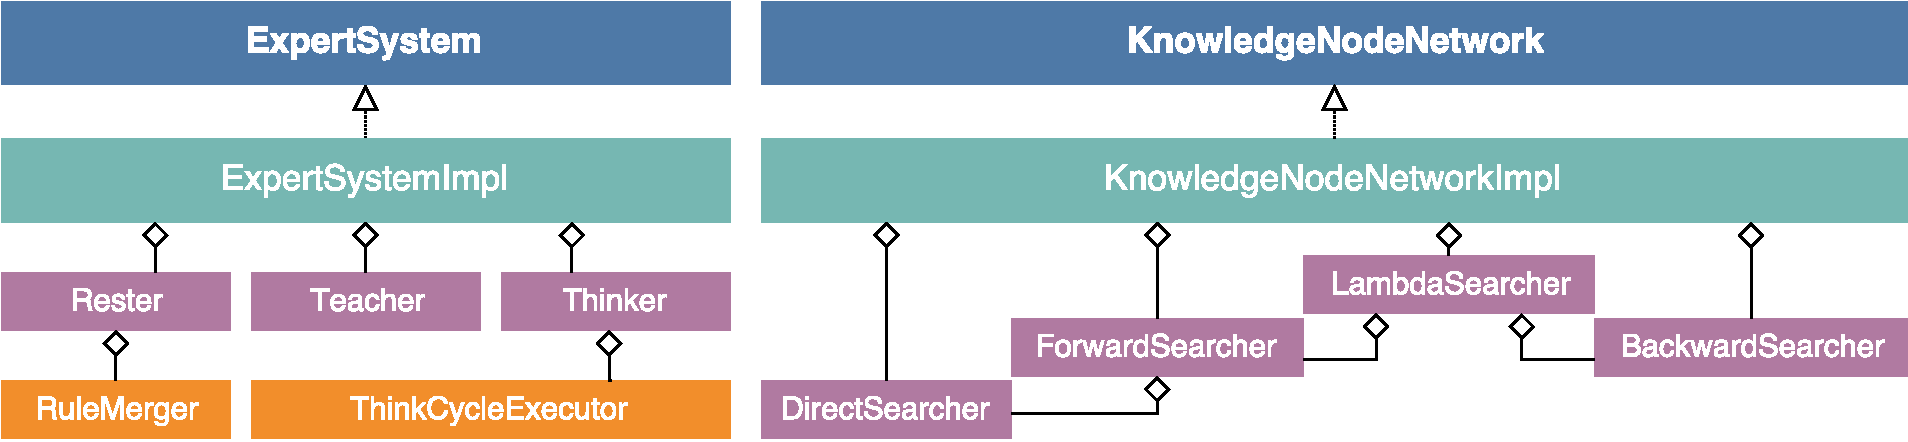
\includegraphics[width=0.99\textwidth]{figures/uml_combined_3.pdf}
						\caption{UML diagrams of the Expert System and KnowledgeNodeNetwork packages.}
					\end{figure}
				
					\parbox{0.99\textwidth}{
					 \textbf{Searching} in the \textbf{Knowledge Node Network} is done by the \code{directSearch()}, \code{forwardSearch()}, \code{backwardSearch()} and \code{lambdaSearch()} methods. These are controlled by the \code{DirectSearcher}, \code{ForwardSearcher}, \code{BackwardSearcher} and \code{LambdaSearcher} classes, respectively. These \textbf{modular} classes allowed great \textbf{re-use}, with the \code{LambdaSearcher} using the \code{ForwardSearcher} and \code{BackwardSearcher}, and the \code{ForwardSeacher} using the \code{DirectSearcher}.}
			
					\begin{figure}
						\centering
						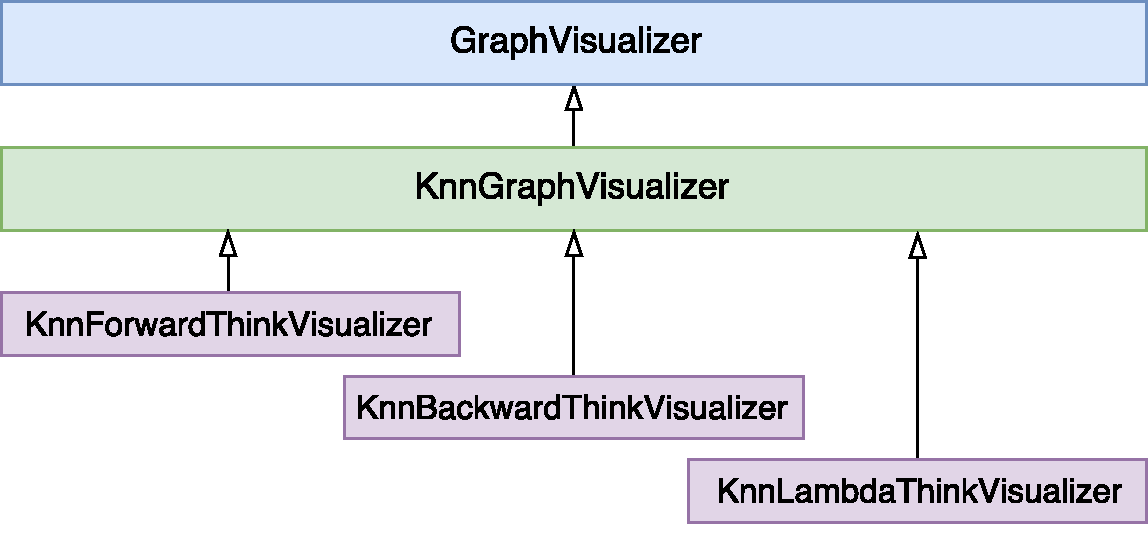
\includegraphics[width=0.6125\textwidth]{figures/uml_graphing.pdf}
						\caption{UML diagram of the graphing package.}
					\end{figure}
				
				\parbox{0.99\textwidth}{
				The Java \textbf{graph visualization} library GraphStream was used to visualize the KNN and the process of searching through it. At each thinking or searching cycle, the graph can be updated in the user-interface and saved to SVG screenshots.}
					
					\begin{figure}[!htb]
						\centering
						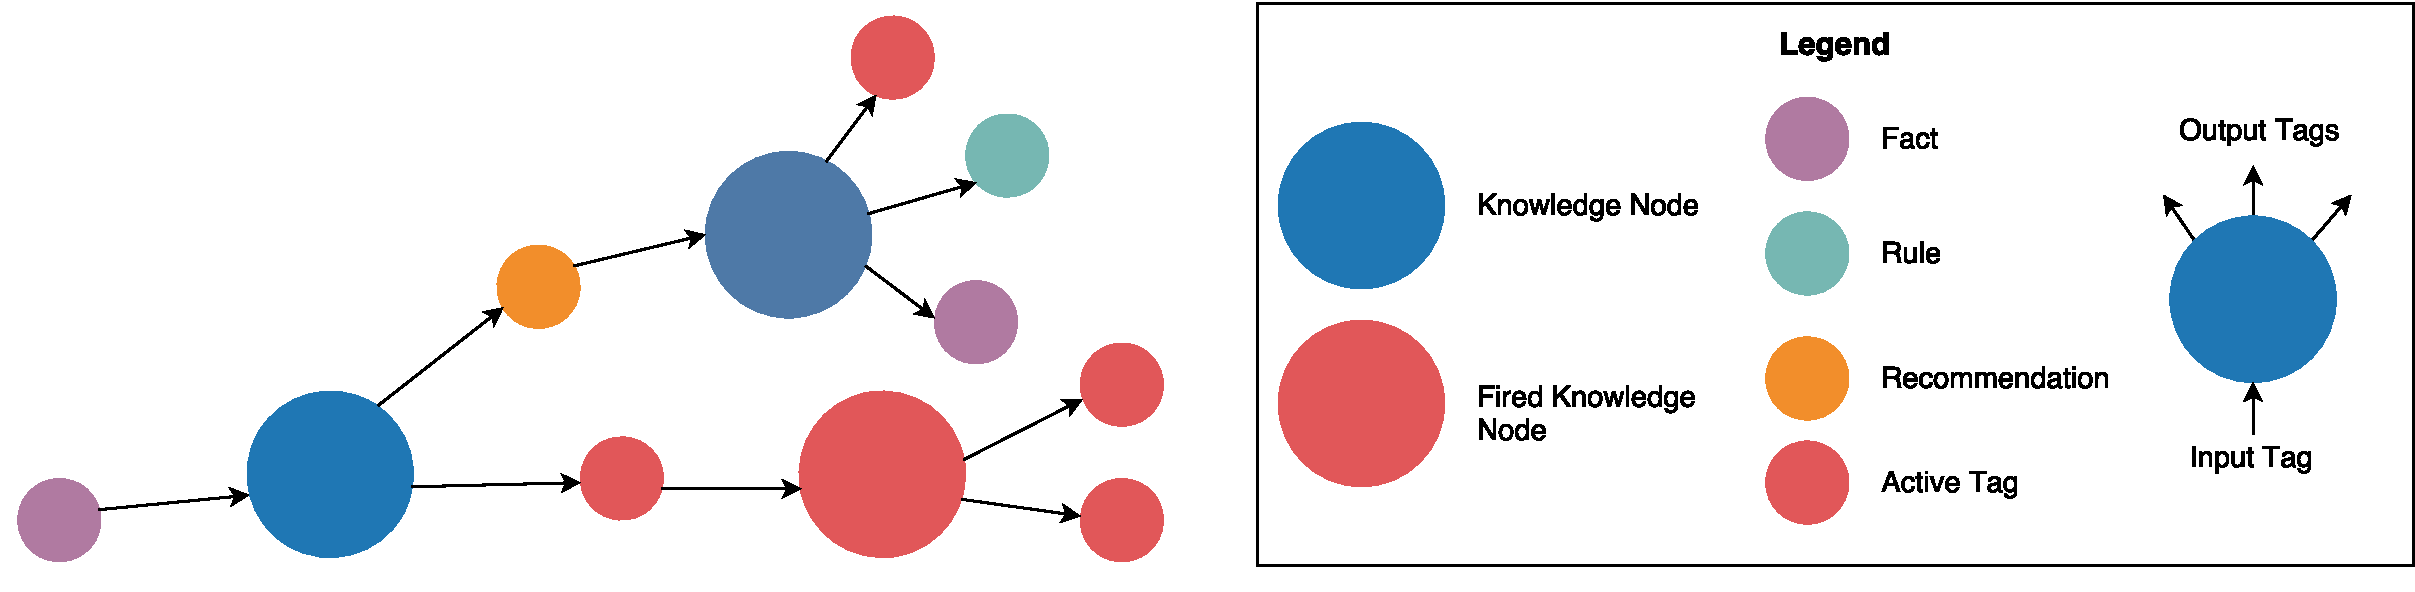
\includegraphics[width=\columnwidth]{figures/knn_graph_legend.pdf}
						\caption
						{Legend for the graph visualization of the KNN.}
						\label{fig:knn_legend}
					\end{figure}
				
				
				\parbox{0.99\textwidth}{
					Prometheus is a Java \textbf{Maven} project, which allows very simple use of many open-source libraries. Some of the libraries used on this project include: \textbf{Google Guice} for modeling and building the dependencies between the layers and their modules, \textbf{Mockito} for mocking objects in unit tests, \textbf{TestNG} for running tests and summarizing their results and \textbf{Apache Commons Lang 3} for standardized \code{toString()}, \code{hashCode()} and \code{equals()} methods.}
					
				\end{block}
				}
			\end{column}
			\begin{column}{.33\textwidth}
				\parbox[t][\columnheight]{\textwidth}{
				\begin{block}{Results \& Tests}
					\parbox{0.99\textwidth}{
						\textbf{Unit tests} were created using \textbf{Mockito} and \textbf{TestNG}. These tests test the functionality of isolated methods. \textbf{Integration tests} were also created with \textbf{TestNG}, testing end-to-end behavior. All of these tests are part of a continuous integration test suite which runs on the GitHub repository whenever a commit is made. This is done using \textbf{Travis CI}. \cref{fig:test_es} shows a simple Expert System integration test.}
					
					\begin{figure}[!htb]
						\centering
						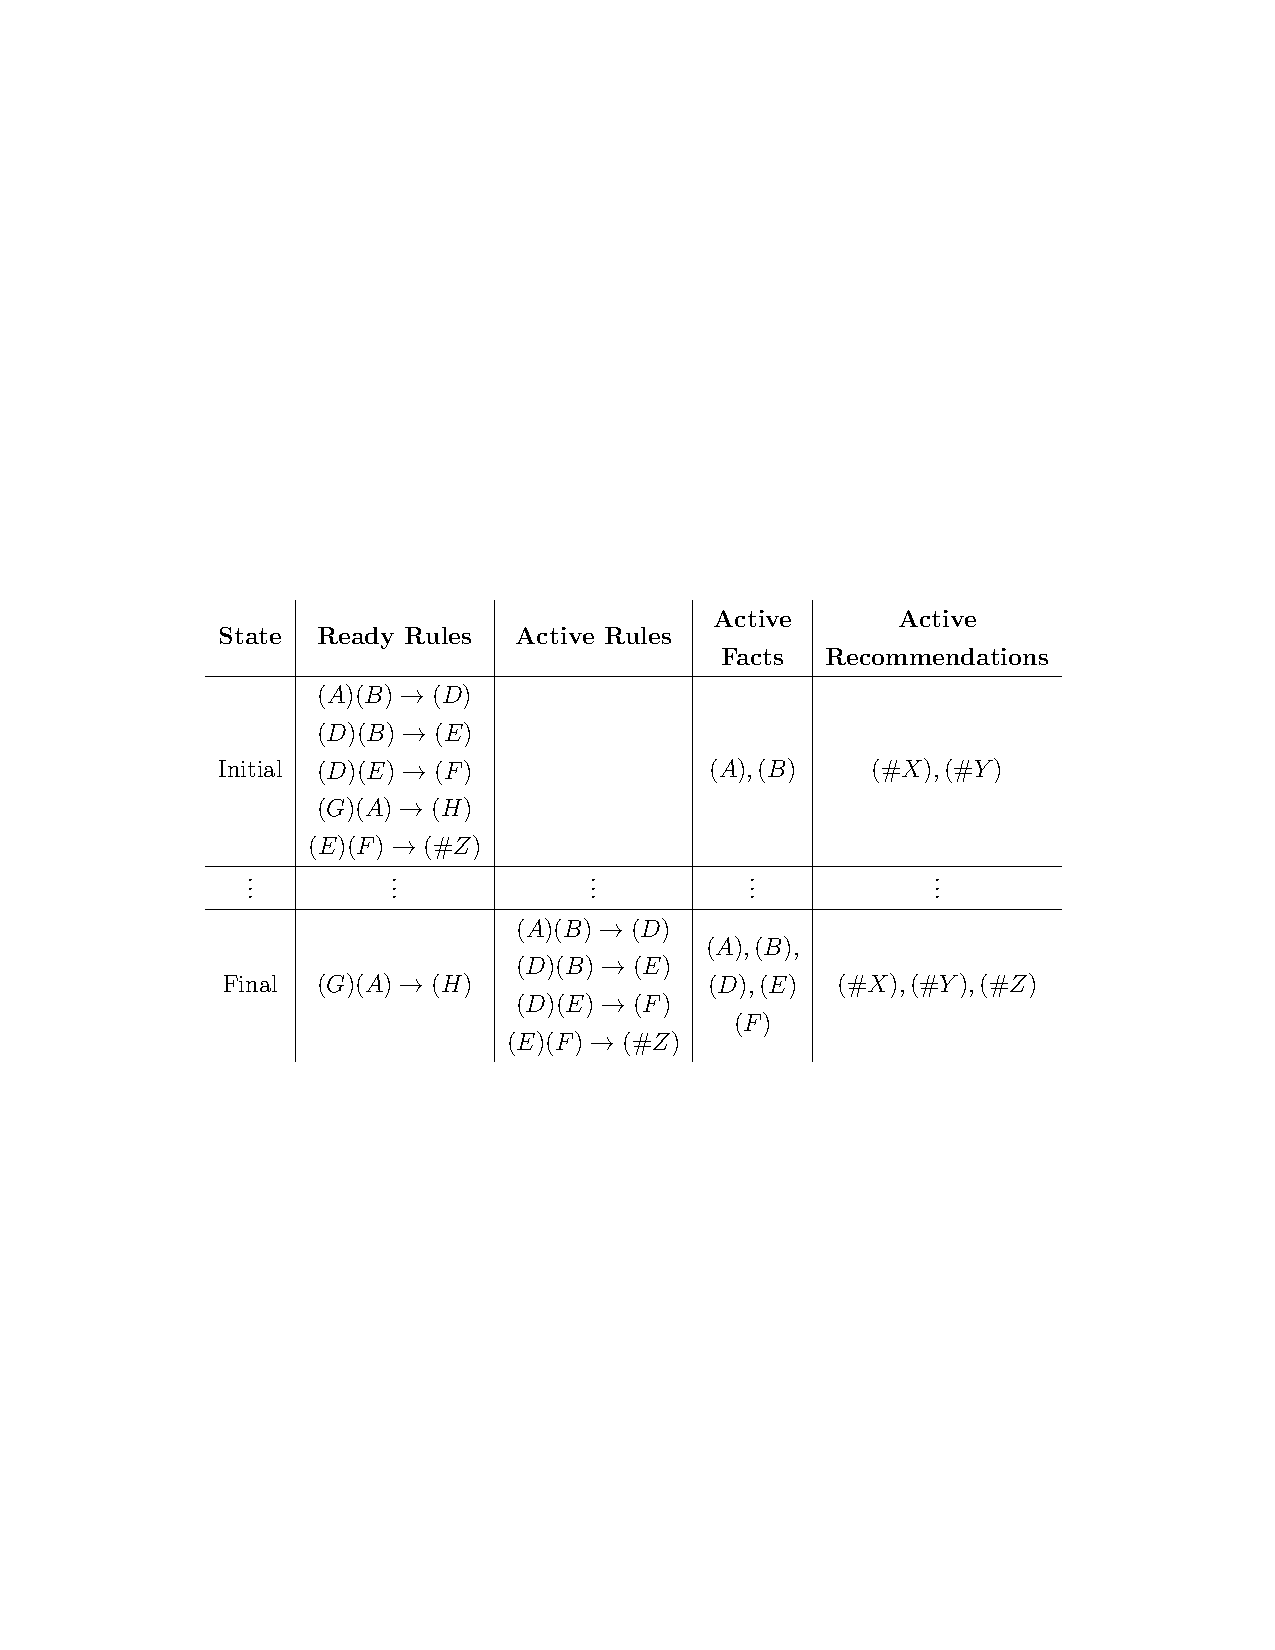
\includegraphics[width=0.7325\textwidth]{figures/testES.pdf}
						\caption
						{ES test setup representing simple rules and facts that must be brought to quiescence.}
						\label{fig:test_es}
					\end{figure}
%					\begin{figure}[!htb]
%						\centering
%						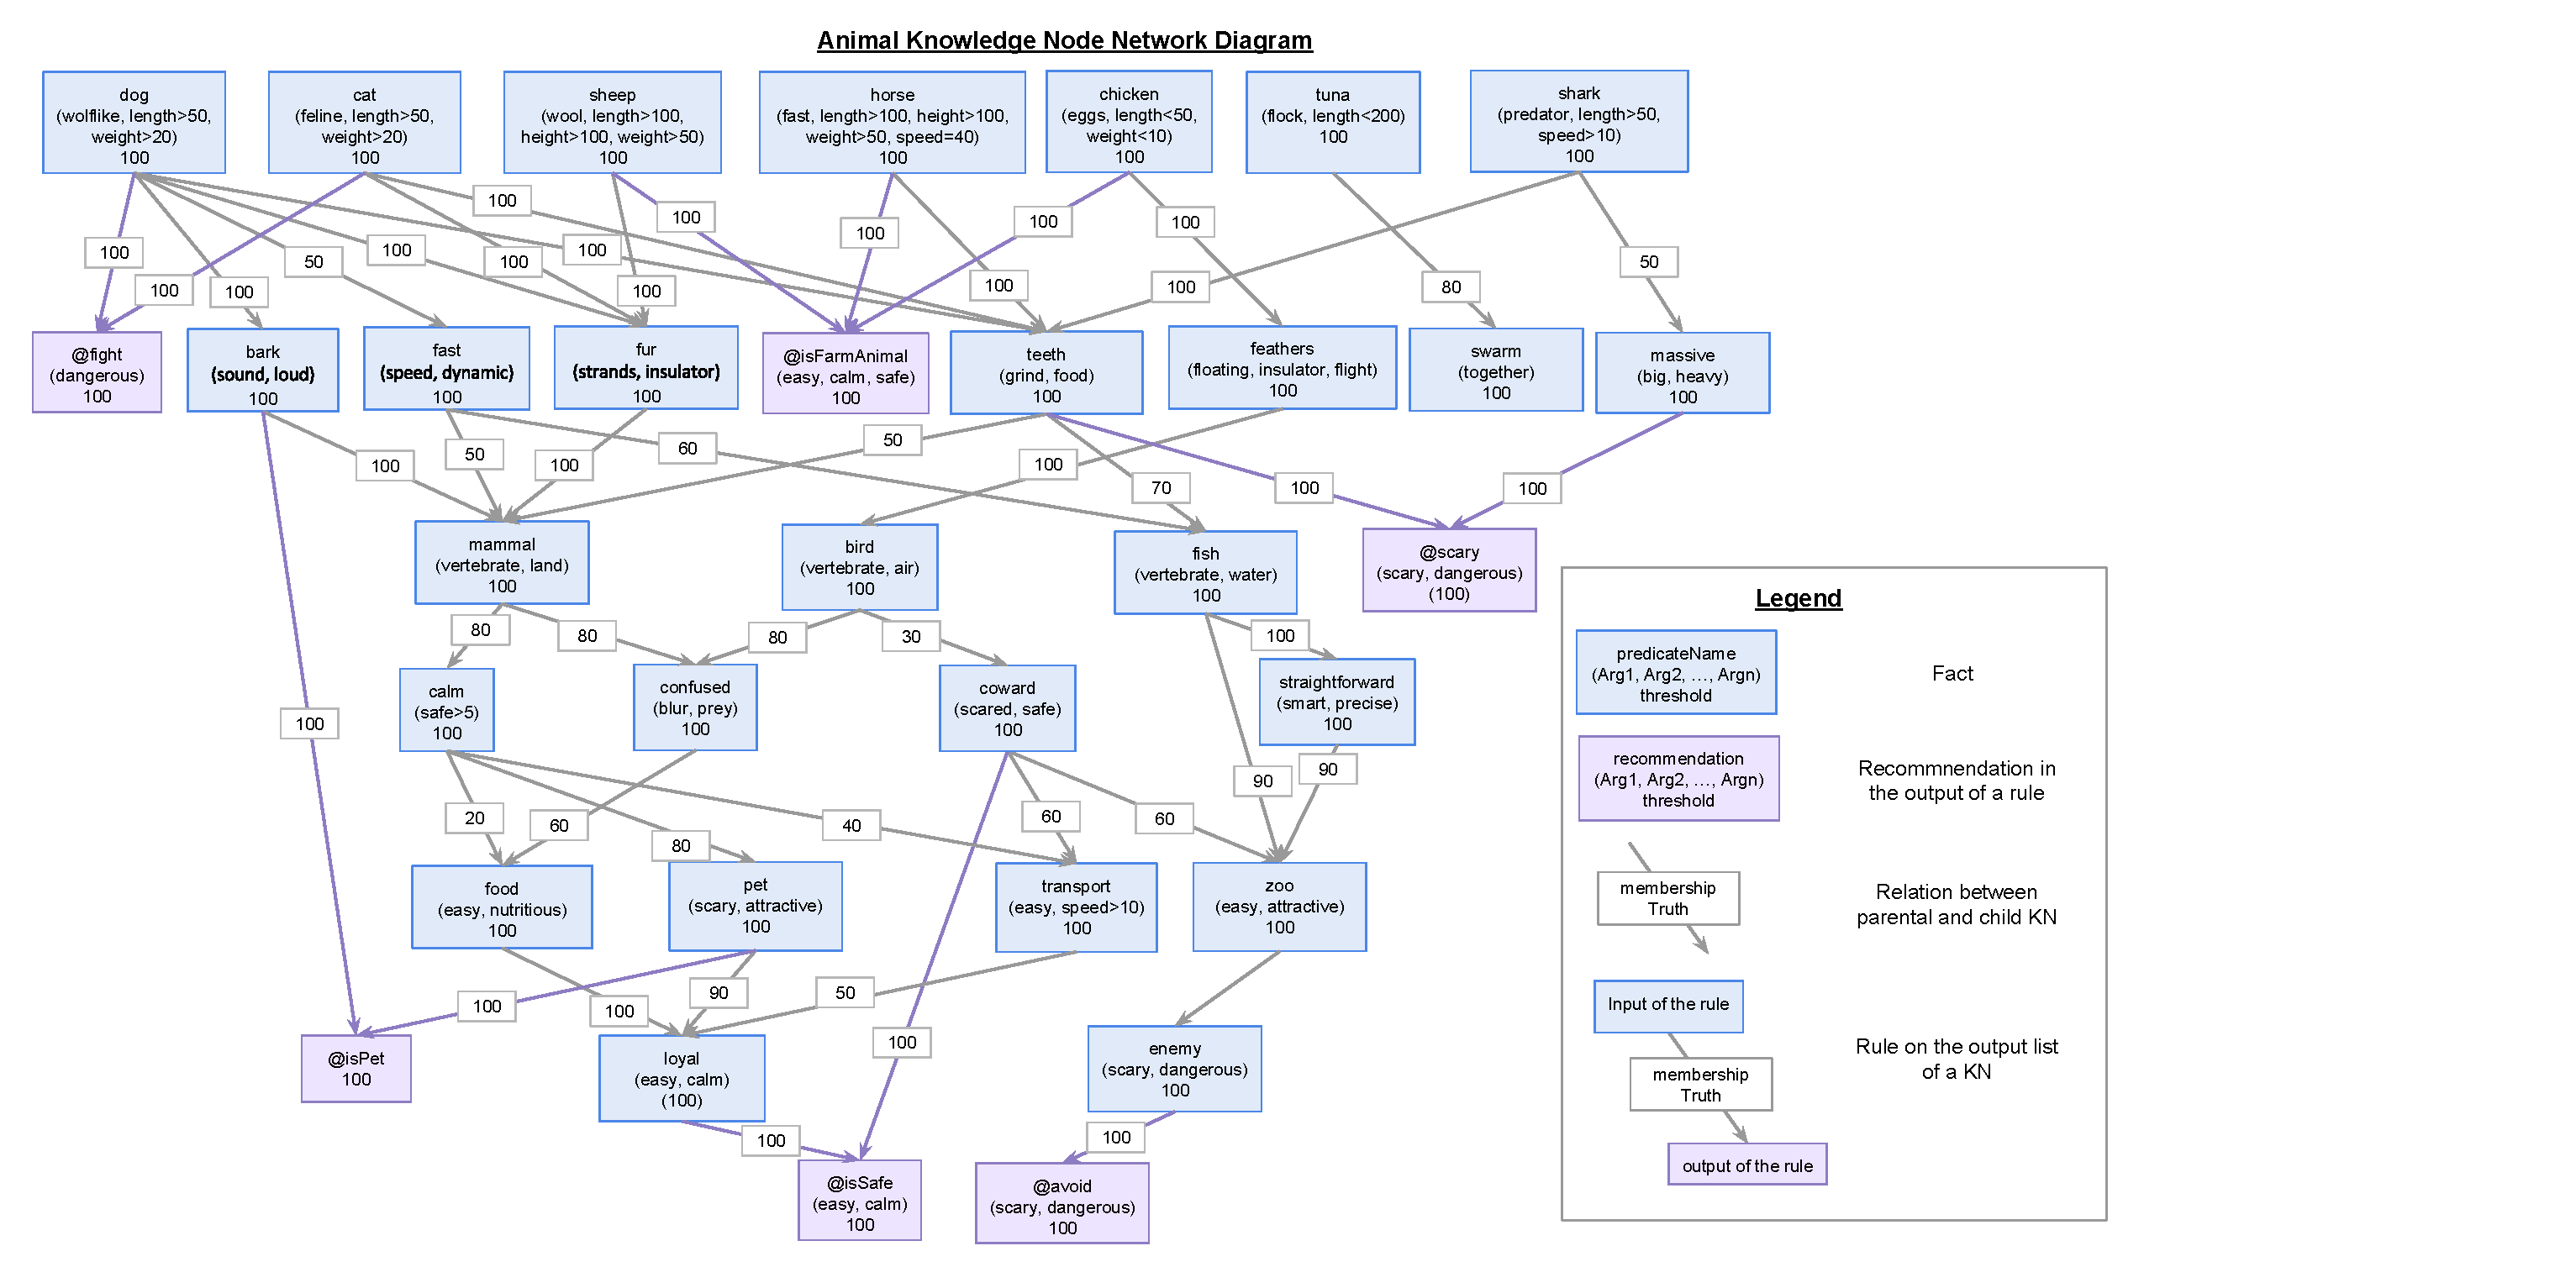
\includegraphics[width=\textwidth]{figures/animal_knn.pdf}
%						\caption
%						{Elaborate test KNN network representing connections between memories of animals and their characteristics. Credit for creating the graph goes to volunteer Laurence Liang.}
%					\end{figure}
					
					\parbox{0.99\textwidth}{The \code{forwardSearch()}, \code{backwardSearch()} and \code{lambdaSearch()} were visualized using the created graph visualization tool. These can be seen in \cref{fig:forward_search_test,fig:backward_search_test,fig:lambda_search_test}. Please refer to \cref{fig:knn_legend} for the meaning of the nodes and their colors.}
					
					\begin{figure}
						\begin{subfigure}[!htb]{0.32\columnwidth}
							\centering
							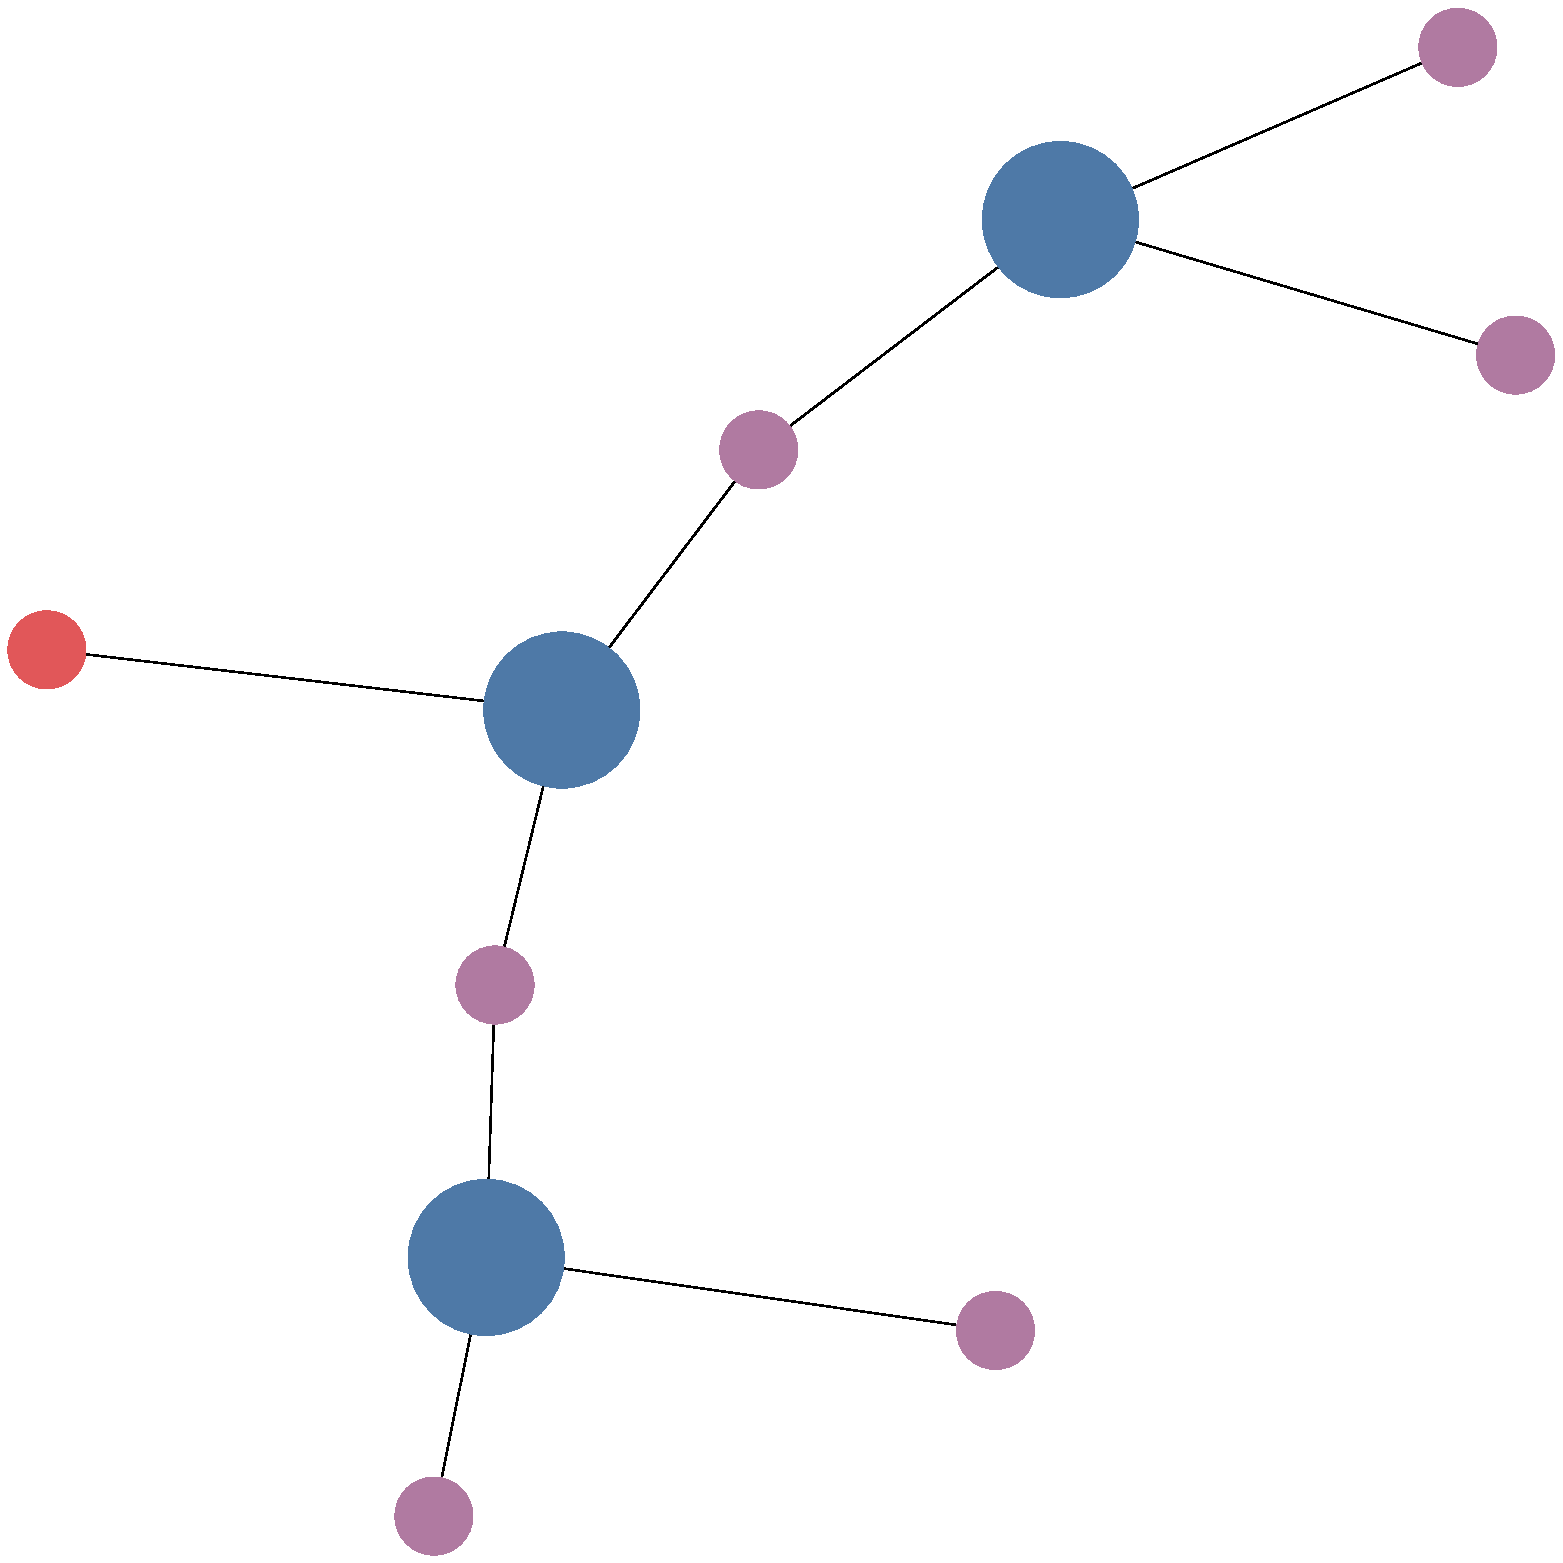
\includegraphics[width=\columnwidth]{figures/knn_simple_forward_think_0.pdf}
							\caption{Ply 0.}
						\end{subfigure}
						\begin{subfigure}[!htb]{0.32\columnwidth}
							\centering
							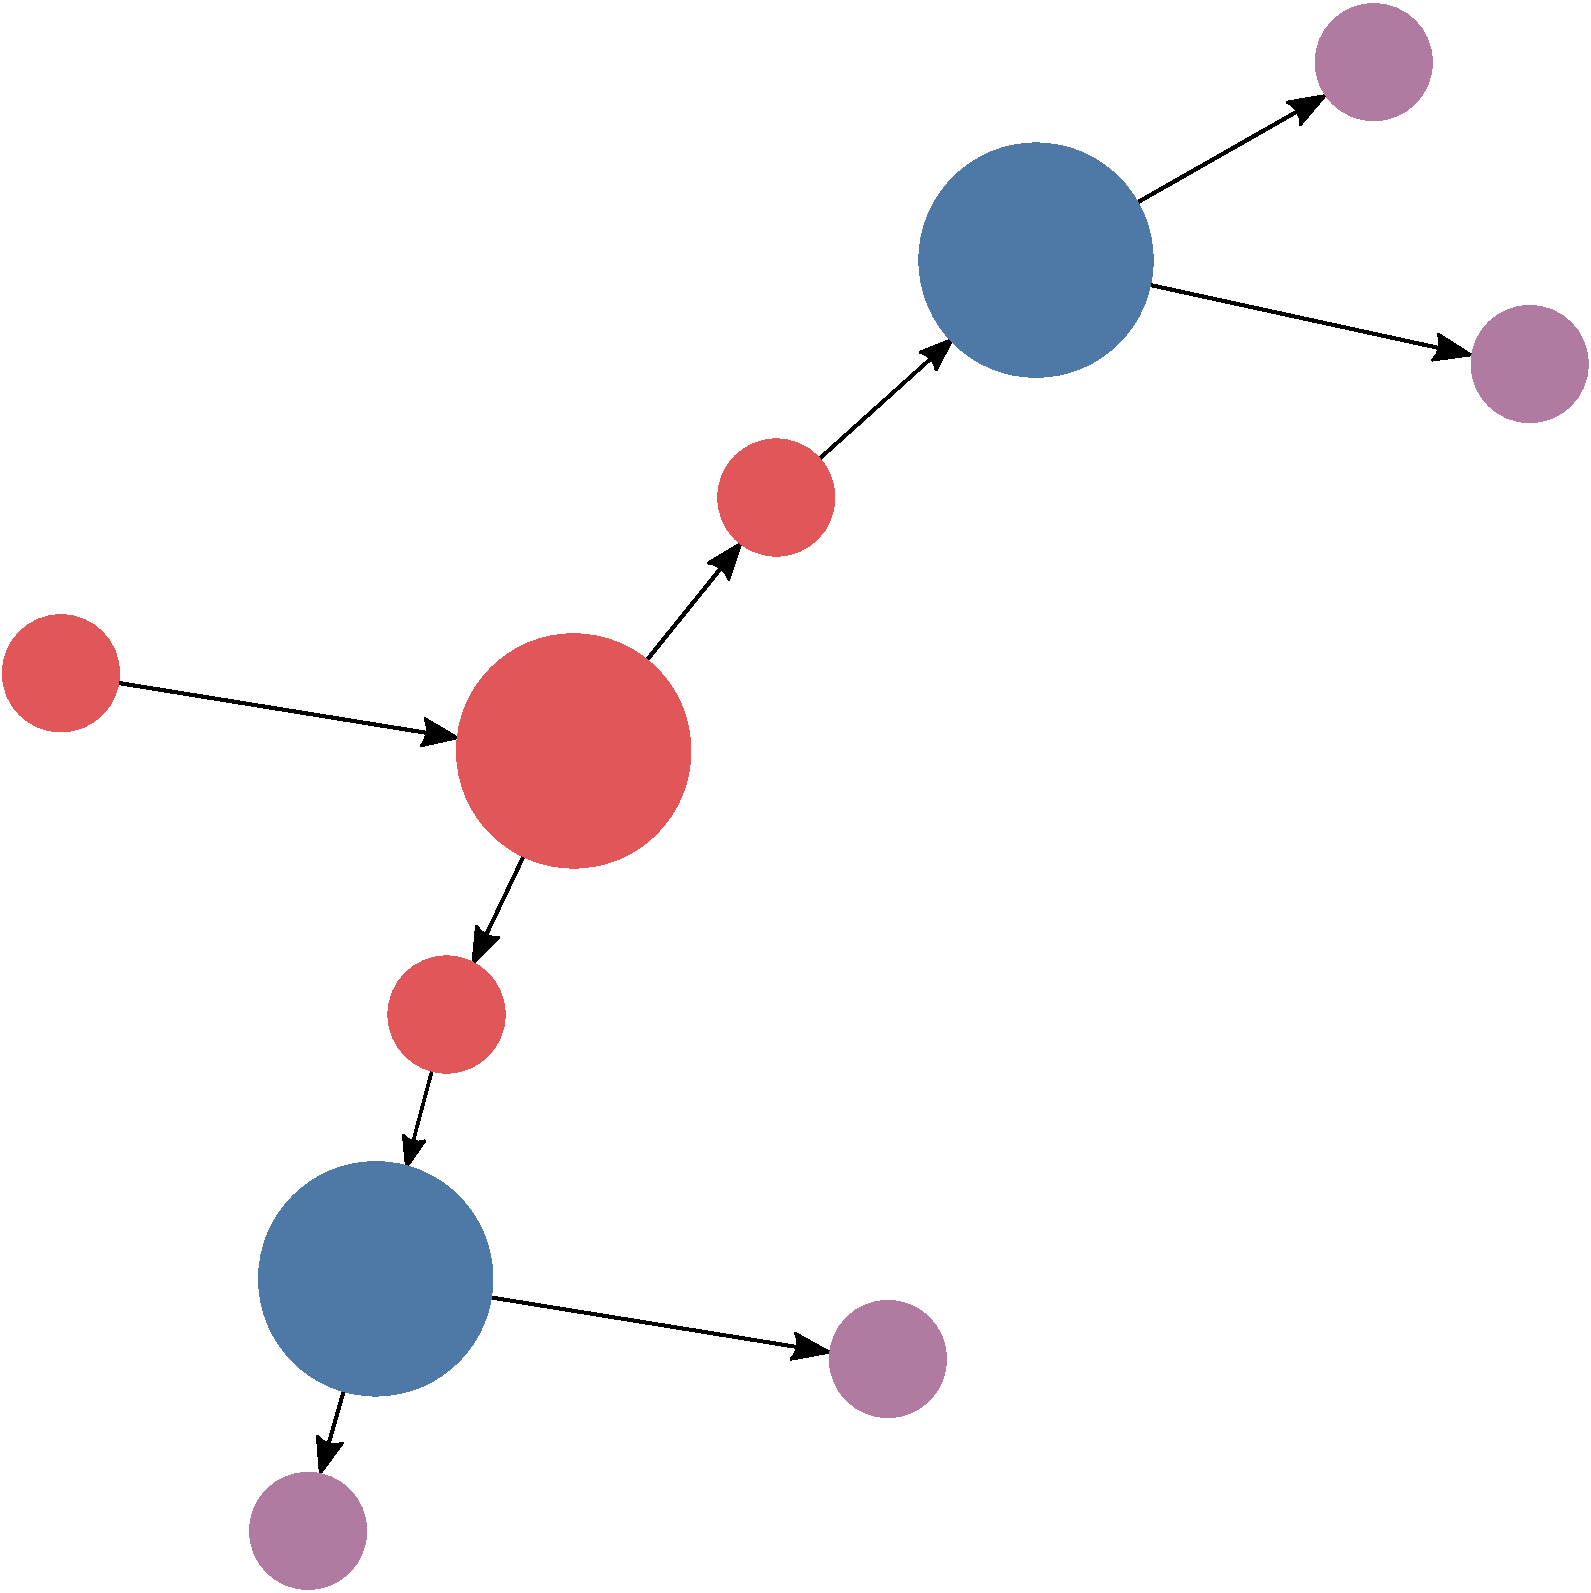
\includegraphics[width=\columnwidth]{figures/knn_simple_forward_think_1.pdf}
							\caption{Ply 1.}
						\end{subfigure}
						\begin{subfigure}[!htb]{0.32\columnwidth}
							\centering
							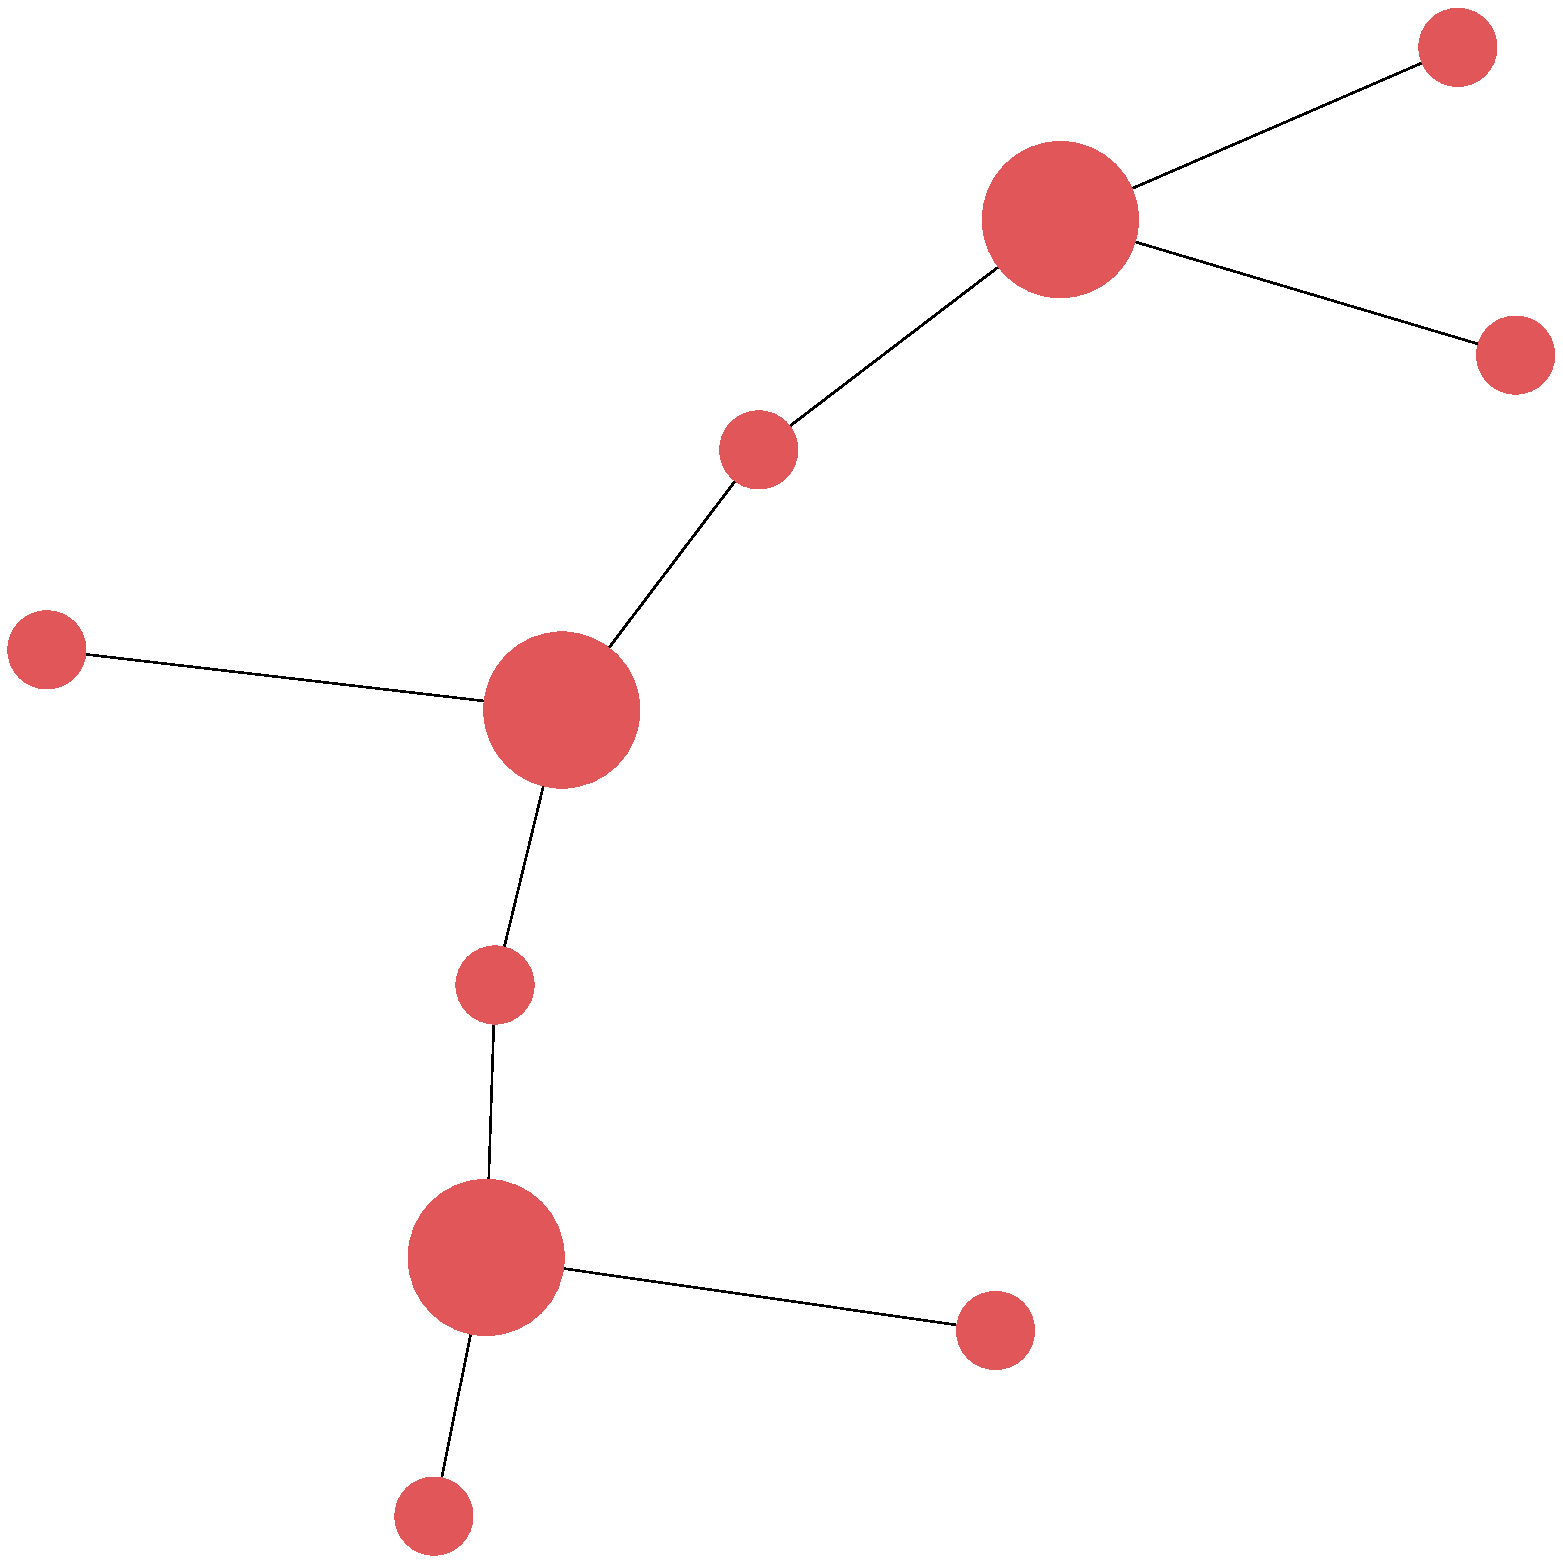
\includegraphics[width=\columnwidth]{figures/knn_simple_forward_think_2.pdf}
							\caption{Ply 2.}
						\end{subfigure}
						\caption{Forward search visualization in the KNN.}
						\label{fig:forward_search_test}
					\end{figure}
					
					\begin{figure}[!htb]
						\centering
						\begin{subfigure}[!htb]{0.32\columnwidth}
							\centering
							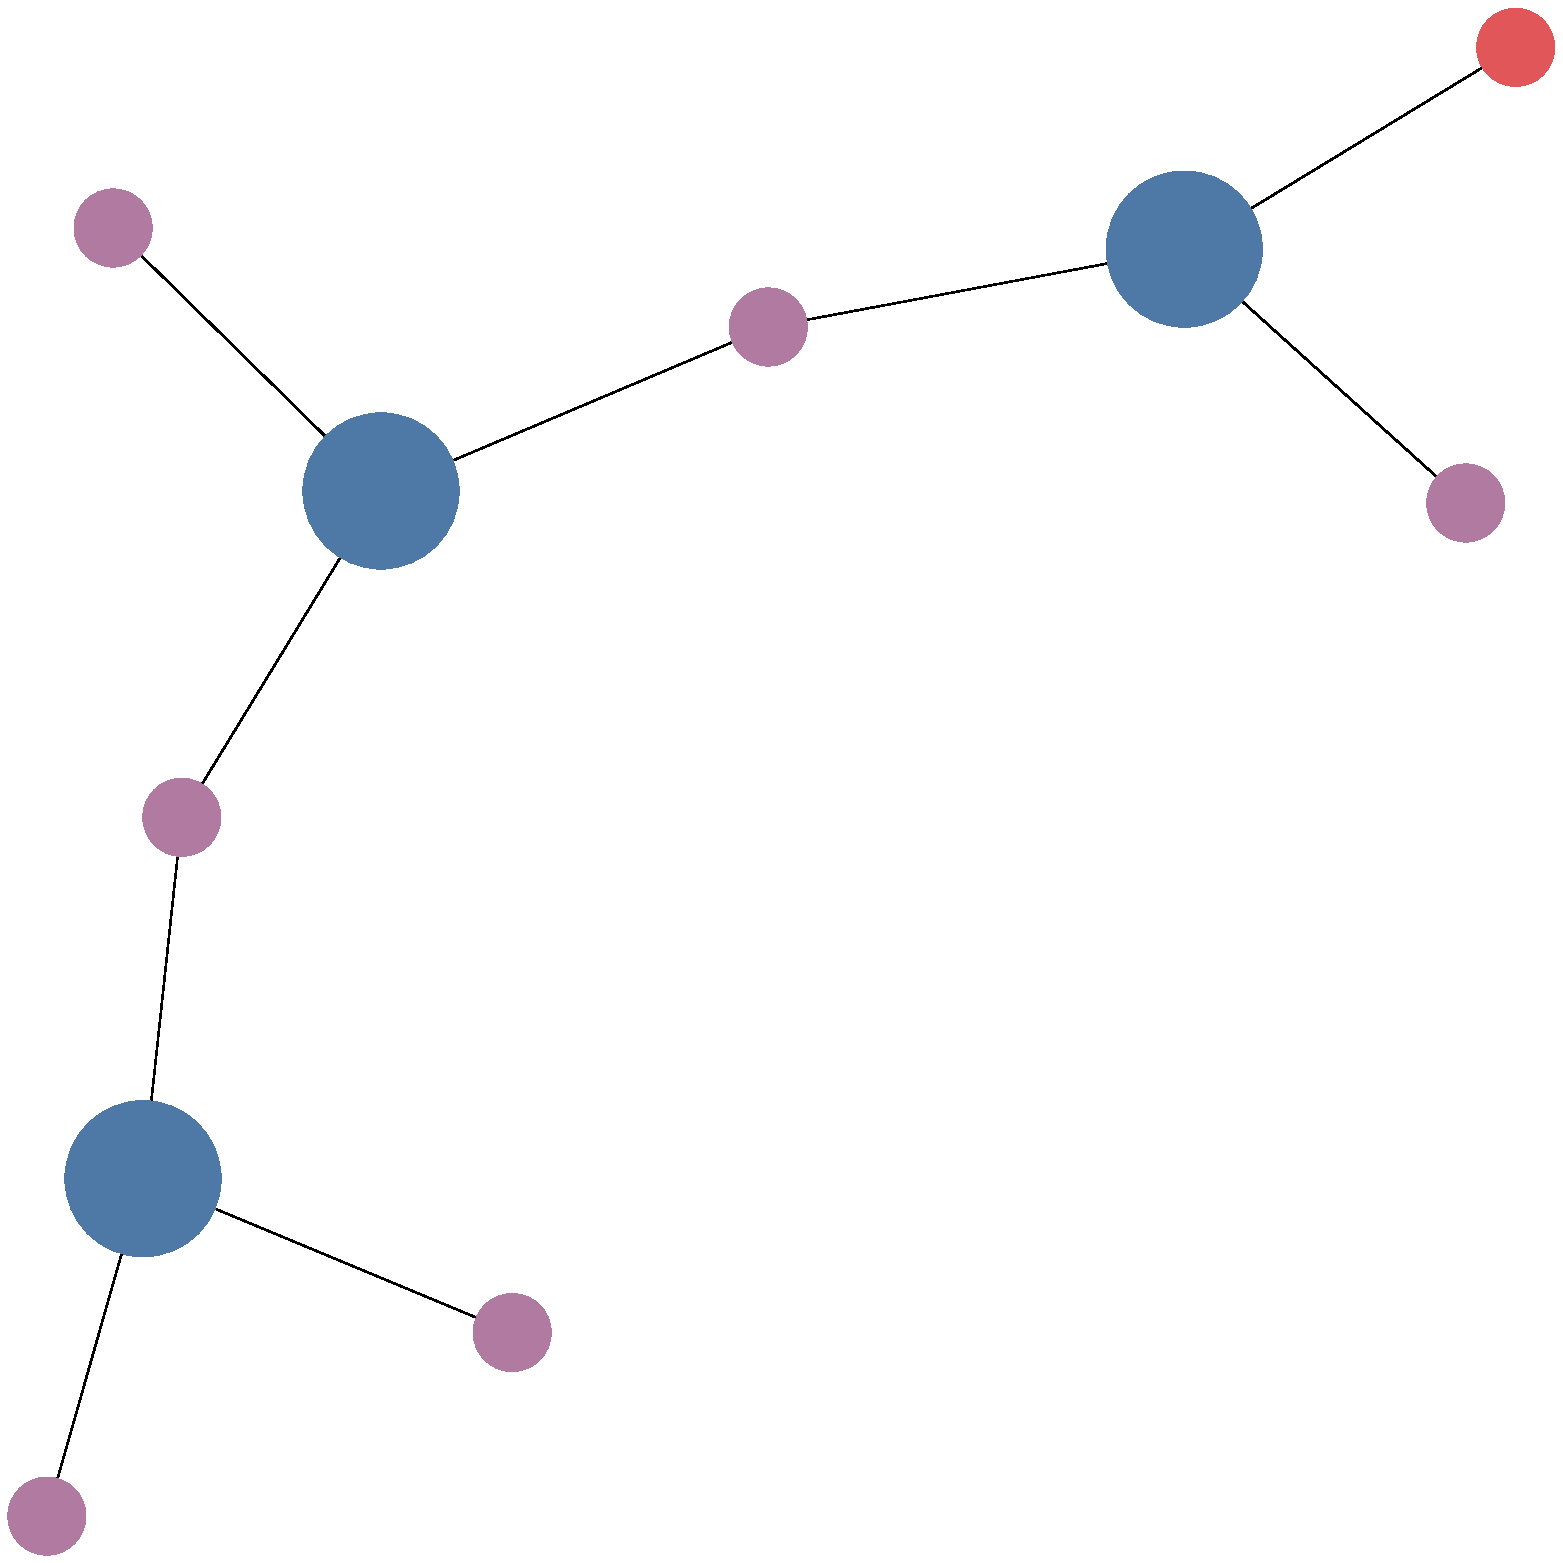
\includegraphics[width=\columnwidth]{figures/knn_simple_backward_think_0.pdf}
							\caption{Ply 0.}
						\end{subfigure}
						\begin{subfigure}[!htb]{0.32\columnwidth}
							\centering
							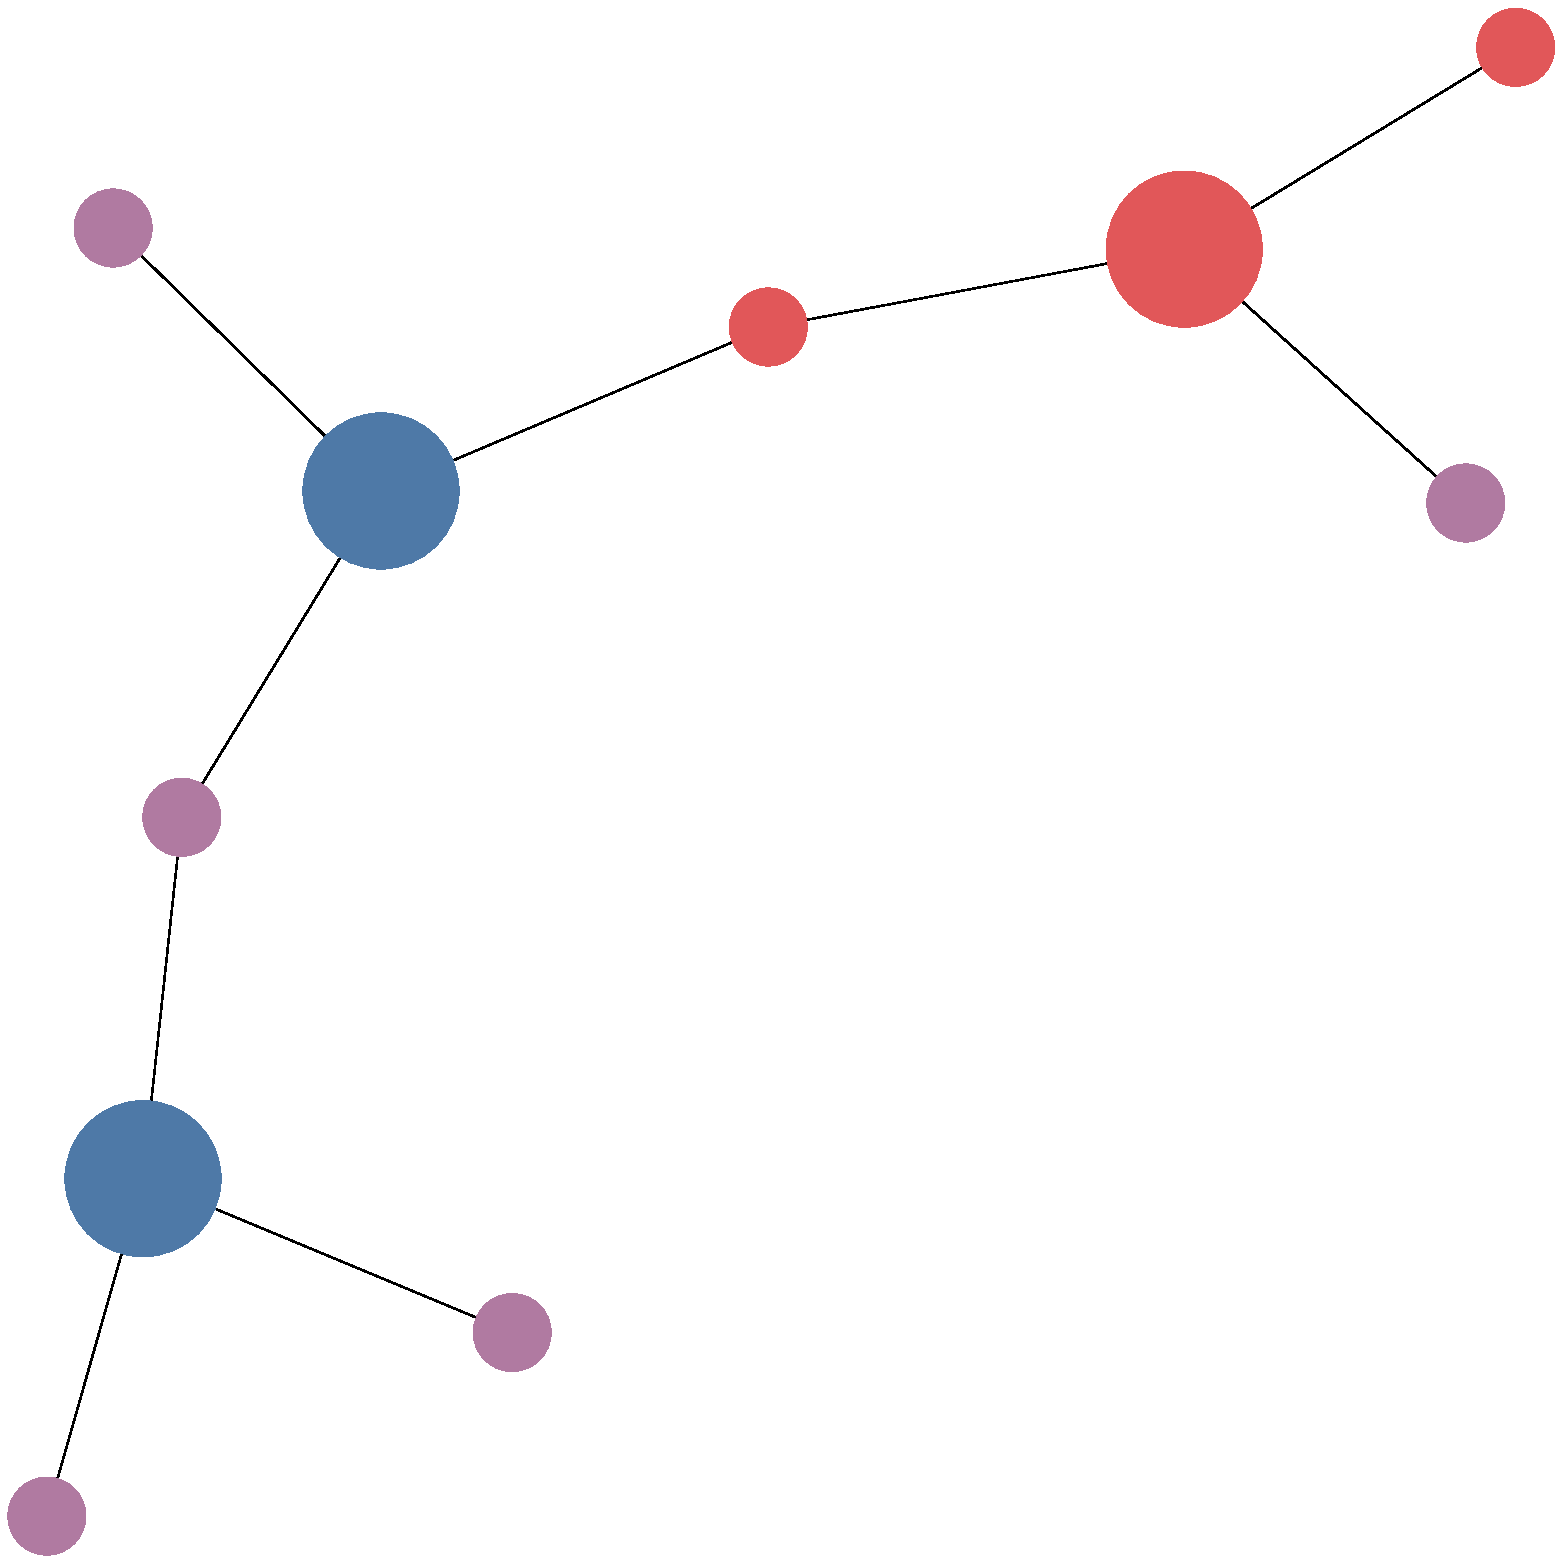
\includegraphics[width=\columnwidth]{figures/knn_simple_backward_think_1.pdf}
							\caption{Ply 1.}
						\end{subfigure}
						\begin{subfigure}[!htb]{0.32\columnwidth}
							\centering
							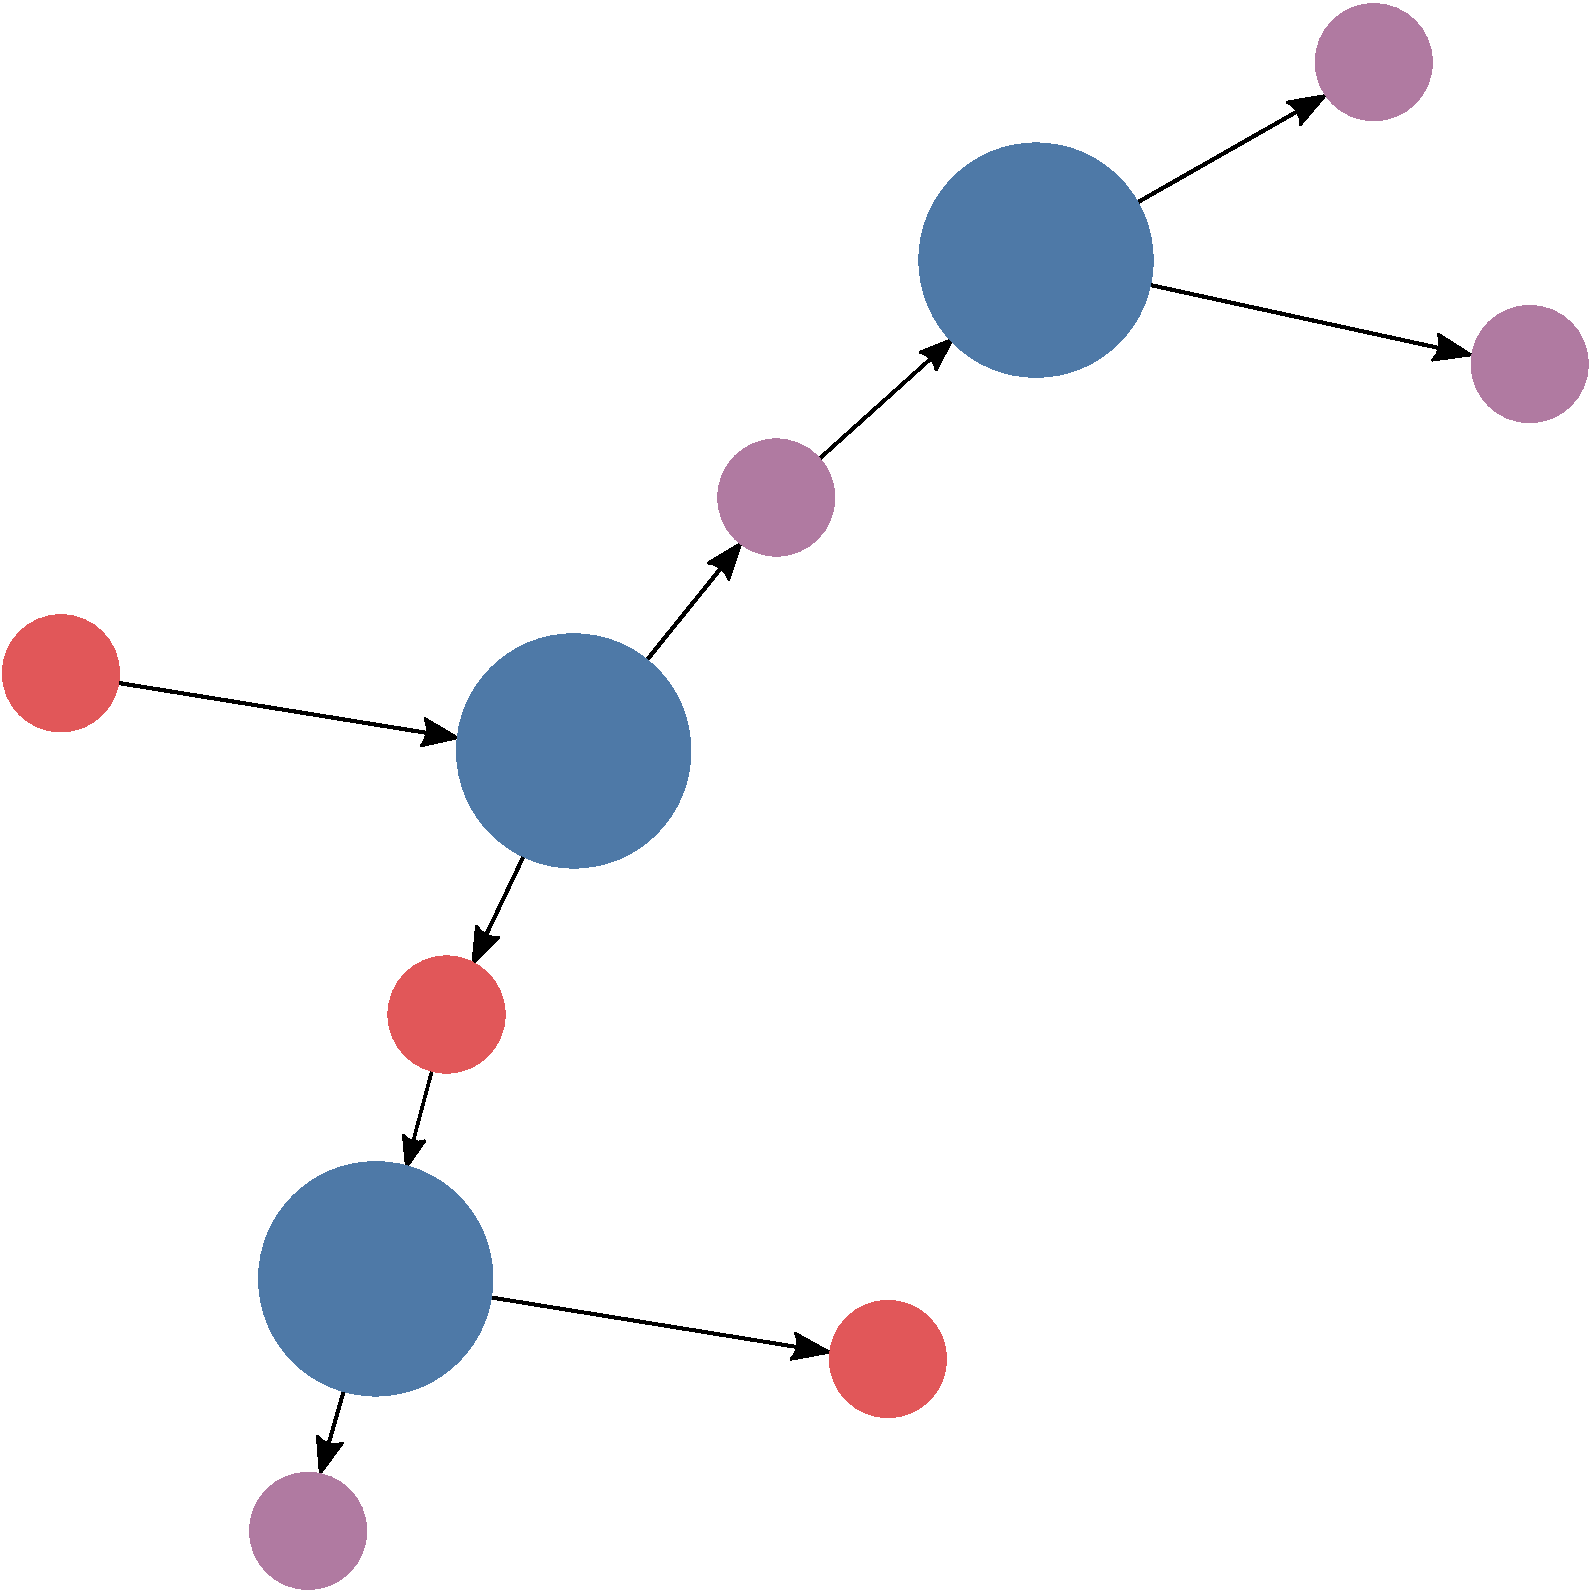
\includegraphics[width=\columnwidth]{figures/knn_simple_backward_think_2.pdf}
							\caption{Ply 2.}
						\end{subfigure}
						\caption{Backward search visualization in the KNN.}
						\label{fig:backward_search_test}
					\end{figure}
				
				
					\begin{figure}[!htb]
						\centering
						\begin{subfigure}[!htb]{0.19\columnwidth}
							\centering
							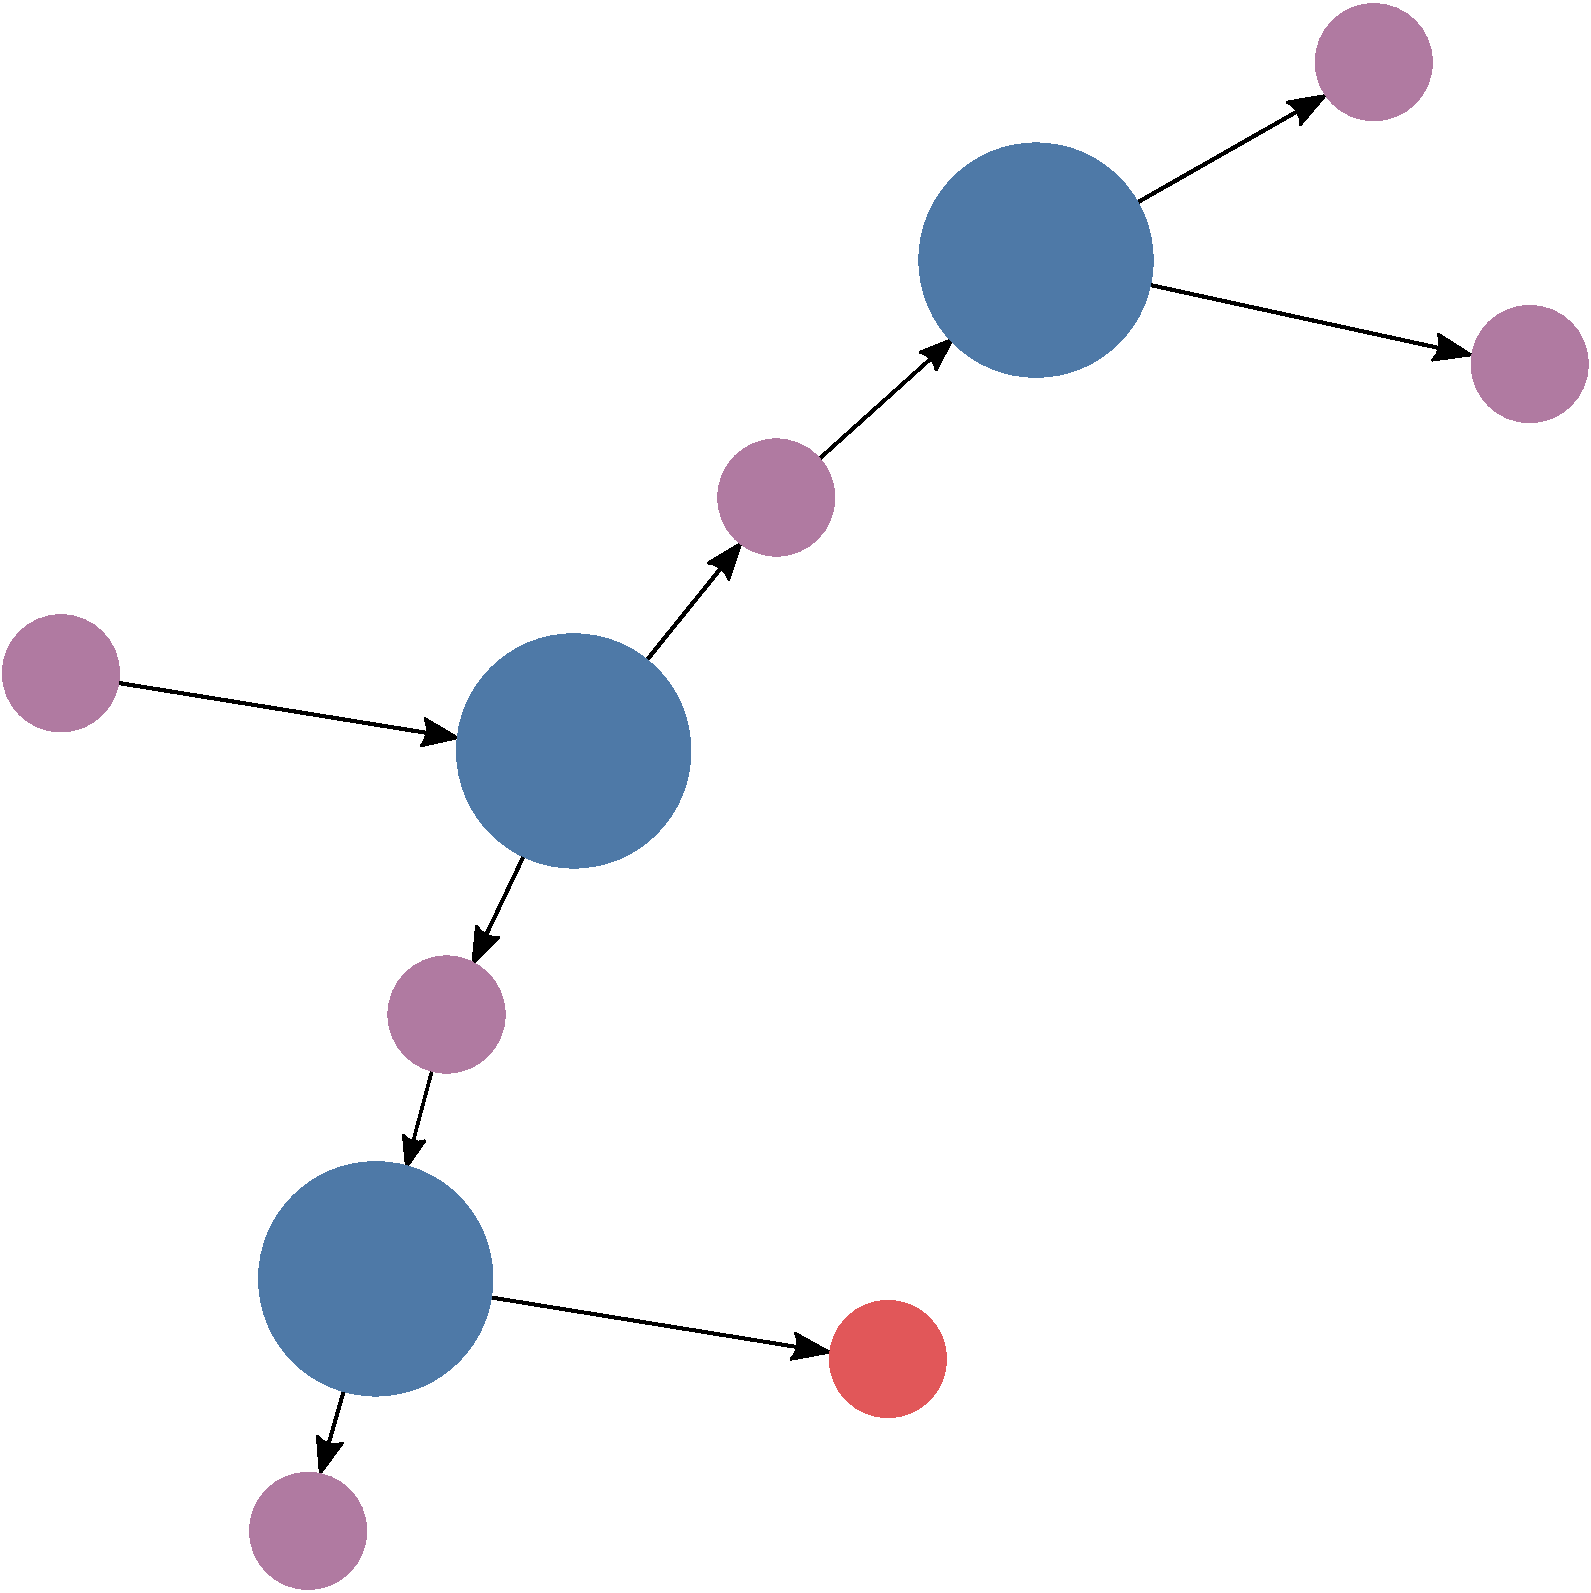
\includegraphics[width=\columnwidth]{figures/knn_simple_lambda_think_0.pdf}
							\caption{Ply 0.}
						\end{subfigure}
						\begin{subfigure}[!htb]{0.19\columnwidth}
							\centering
							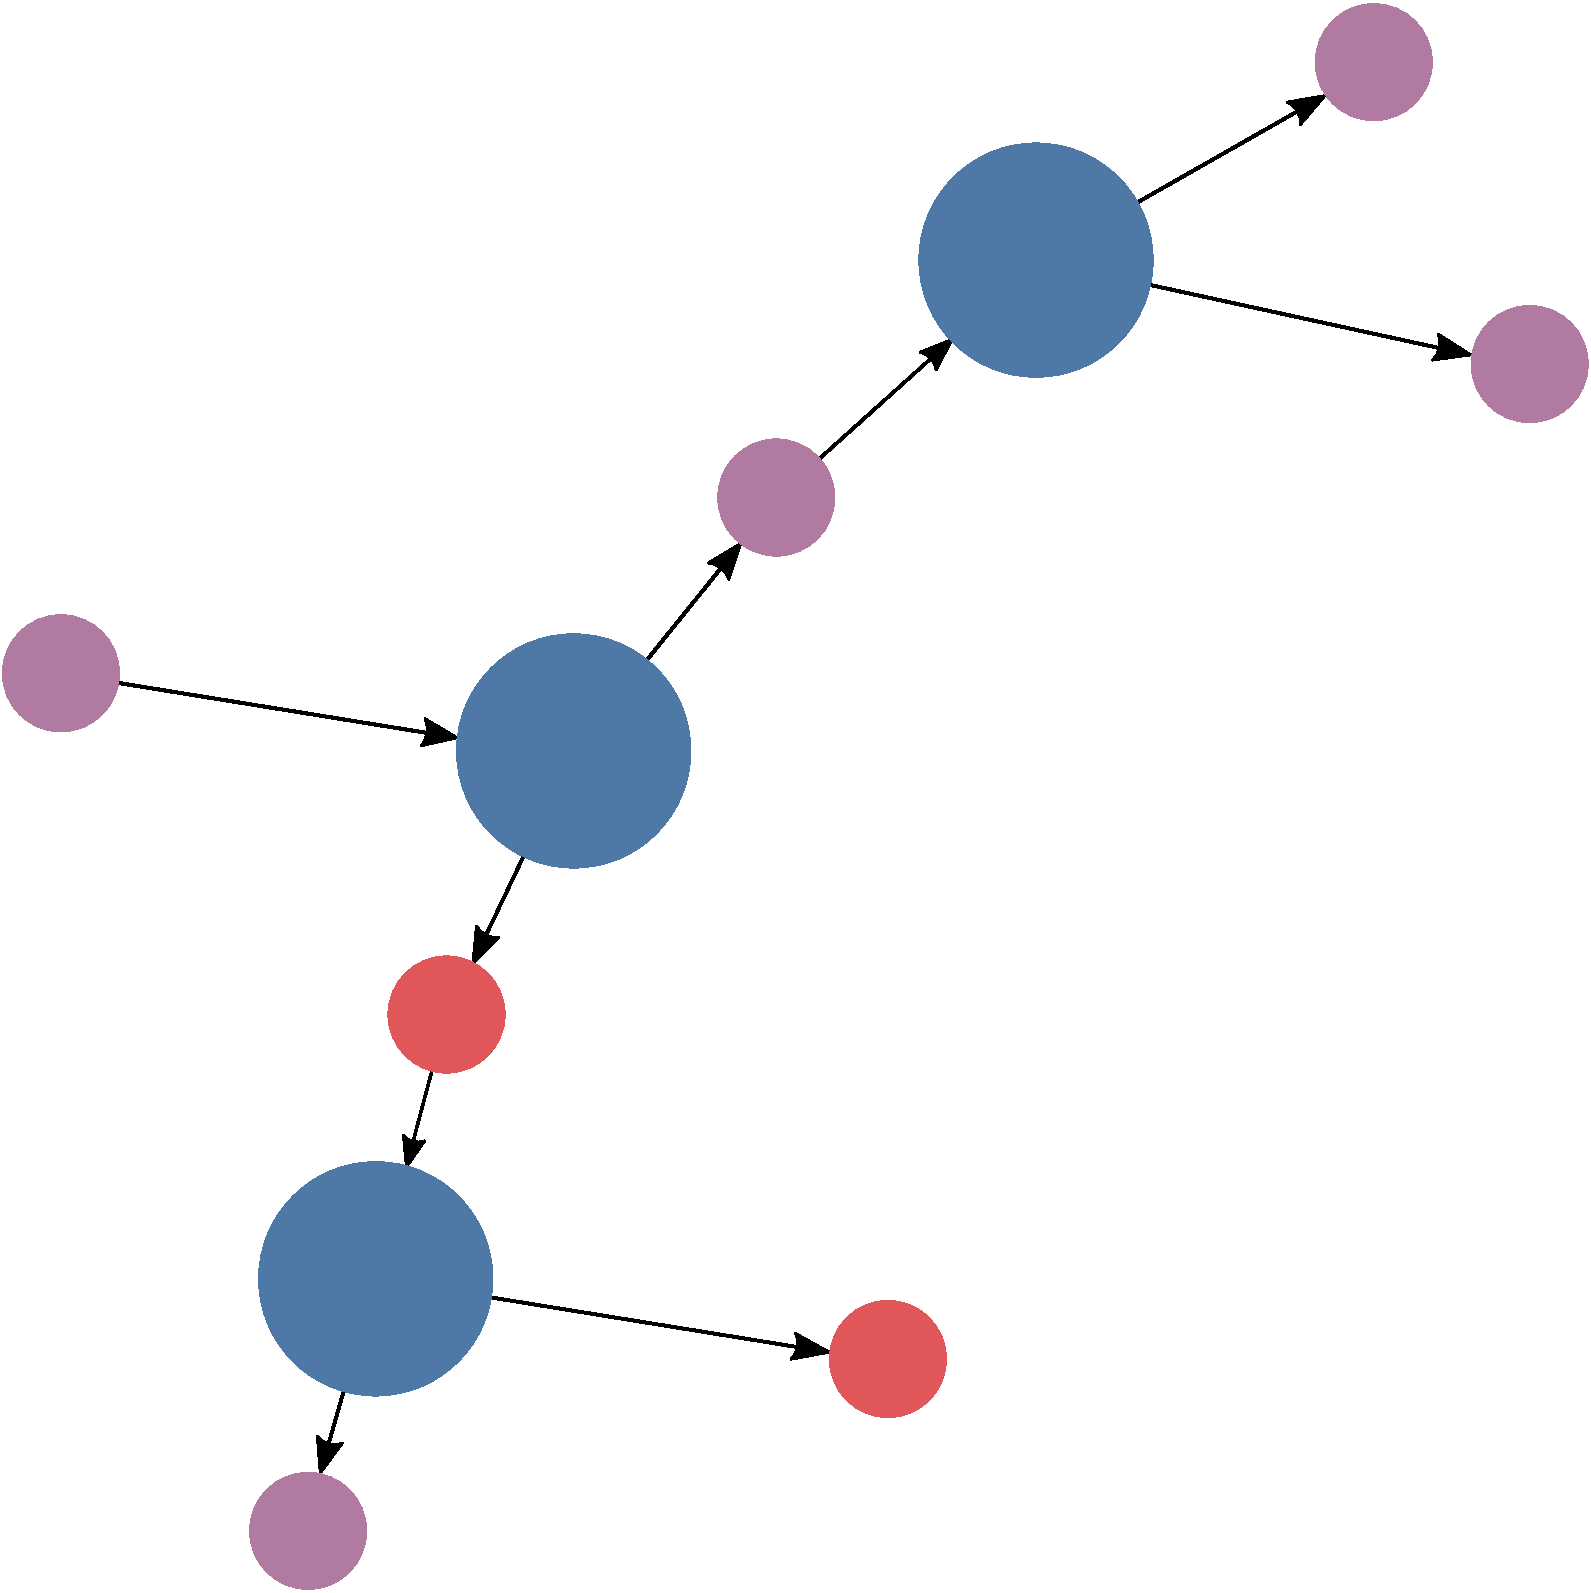
\includegraphics[width=\columnwidth]{figures/knn_simple_lambda_think_1.pdf}
							\caption{Ply 1.}
						\end{subfigure}
						\begin{subfigure}[!htb]{0.19\columnwidth}
							\centering
							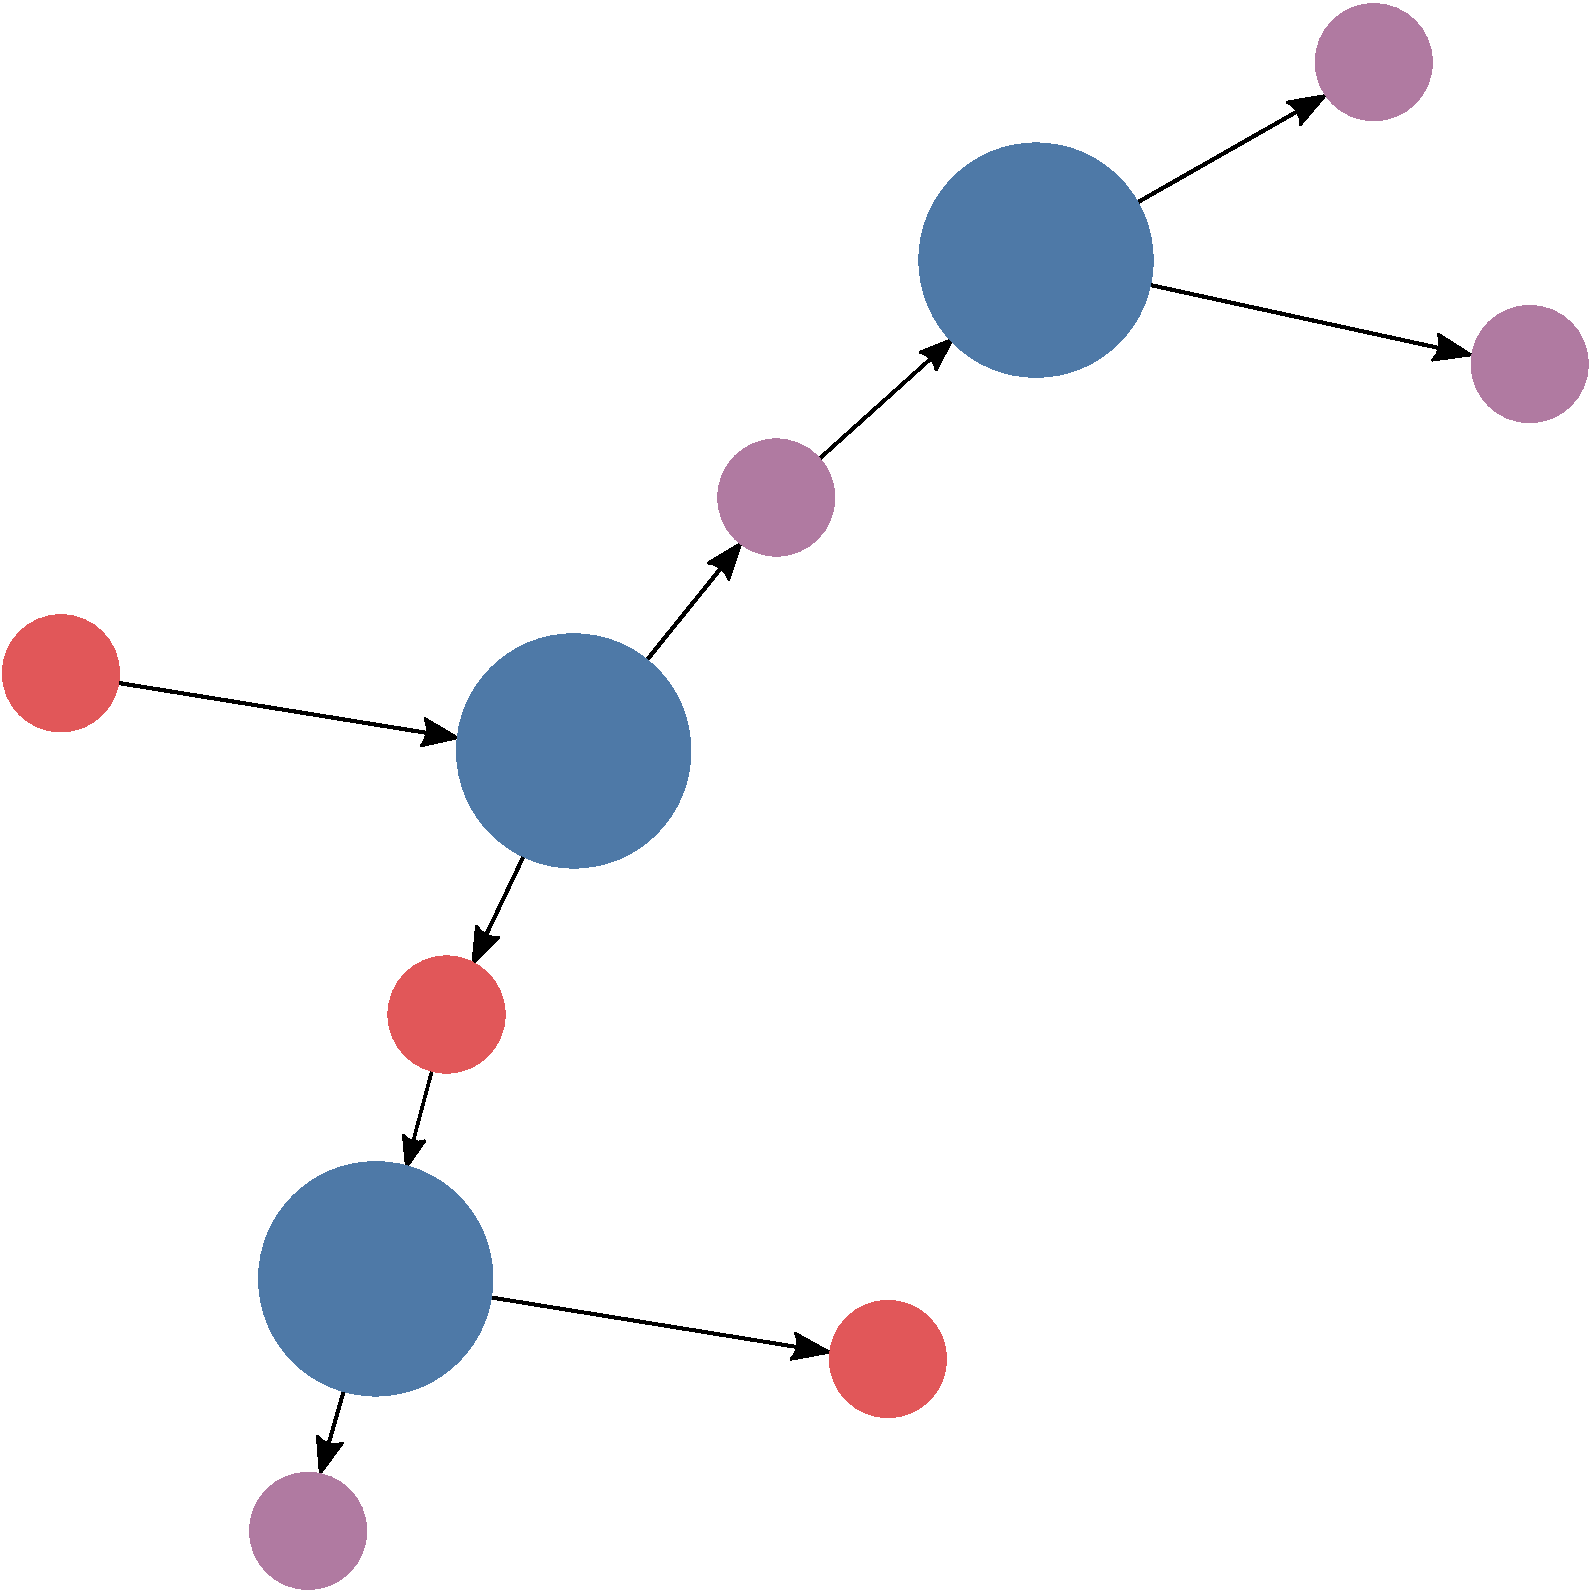
\includegraphics[width=\columnwidth]{figures/knn_simple_lambda_think_2.pdf}
							\caption{Ply 2.}
						\end{subfigure}
						\begin{subfigure}[!htb]{0.19\columnwidth}
							\centering
							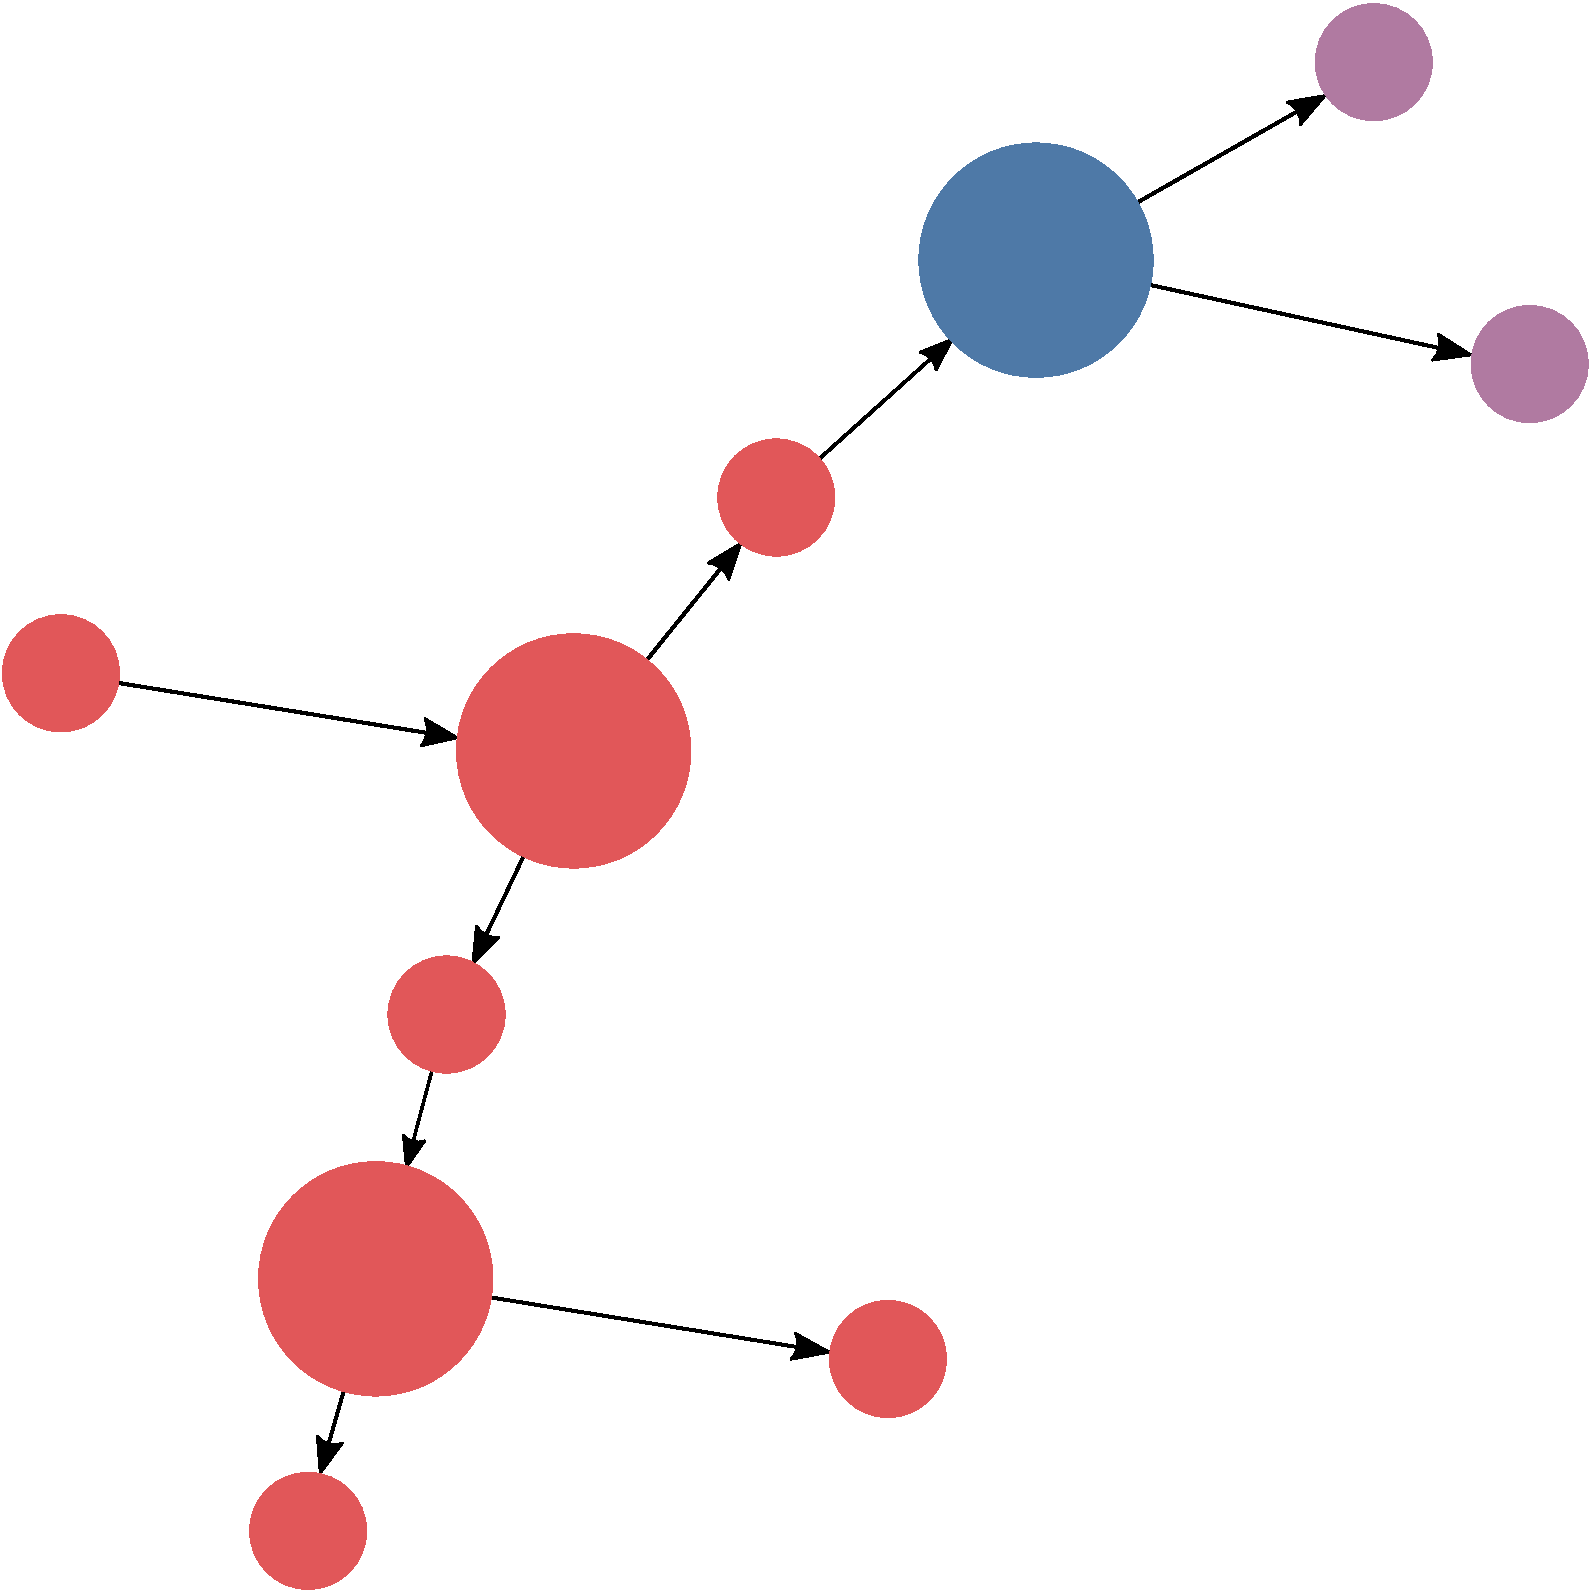
\includegraphics[width=\columnwidth]{figures/knn_simple_lambda_think_3.pdf}
							\caption{Ply 3.}
						\end{subfigure}
						\begin{subfigure}[!htb]{0.19\columnwidth}
							\centering
							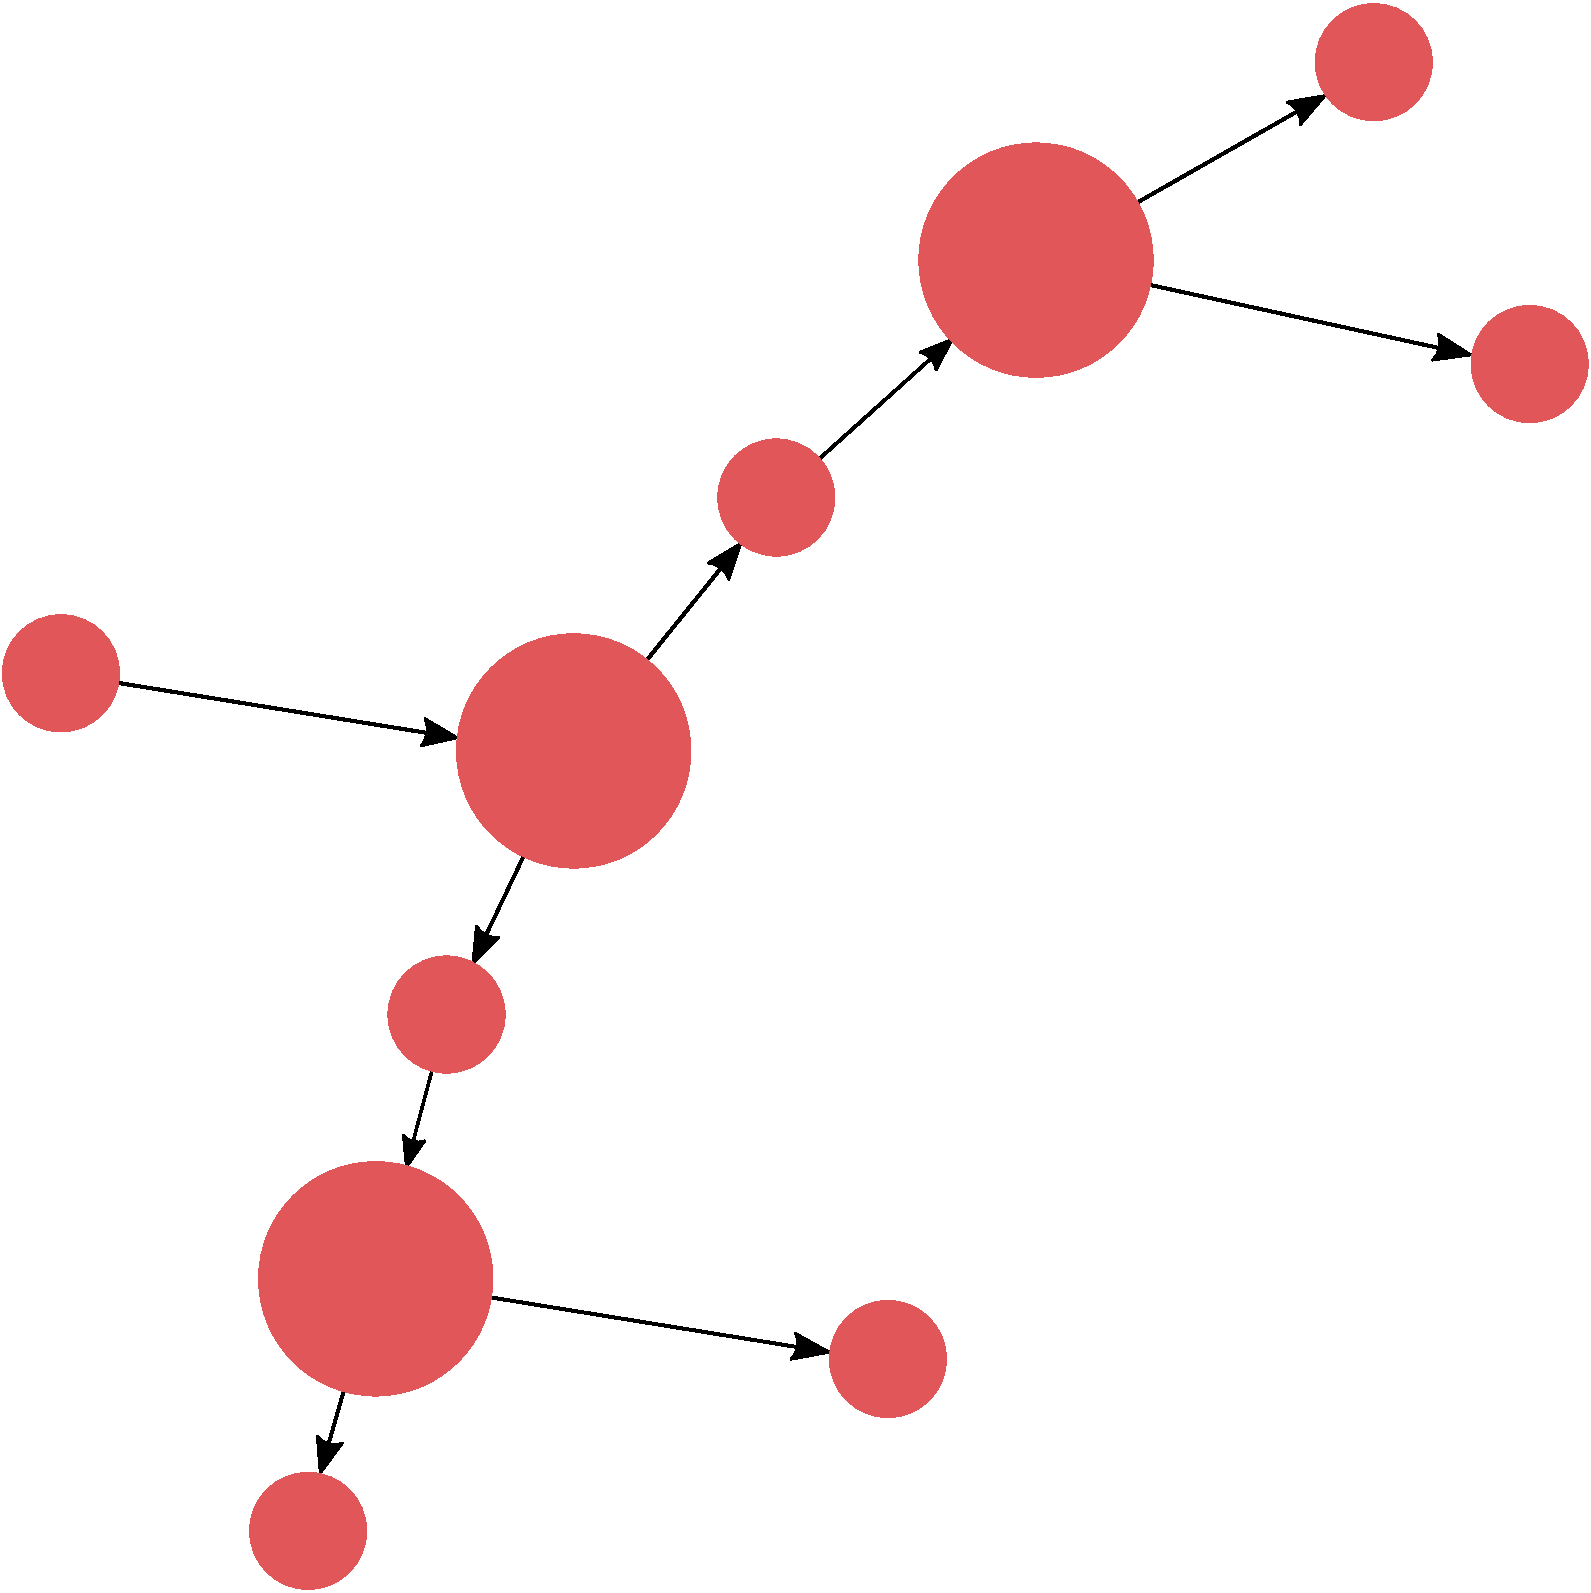
\includegraphics[width=\columnwidth]{figures/knn_simple_lambda_think_4.pdf}
							\caption{Ply 4.}
						\end{subfigure}
						\caption{Lambda search visualization in the KNN.}
						\label{fig:lambda_search_test}
					\end{figure}
				
				\end{block}
				\begin{block}{Conclusion}
					\parbox{0.99\textwidth}{
						Over the course of this project, I learned a great deal of skills relating to \textbf{designing} and \textbf{implementing} large-scale software projects, specifically with Java. I also learned a great deal about various \textbf{cognitive science} topics relating to Prometheus. Finally, setting up systems for software project \textbf{collaboration} was also learned. Possible further work relating to this project could be implementing the missing \textbf{NN} and \textbf{META} layers, as well as implementing more features in the KNN, such as \textbf{learning} and \textbf{attention}.}
				\end{block}
			}
			\end{column}
		\end{columns}
	\end{frame}
\end{document}